\documentclass[a4paper,11pt]{article}
\usepackage[T1]{fontenc}
\usepackage[utf8]{inputenc}
\usepackage[slovak]{babel}
\usepackage{textcomp}
\usepackage{graphicx}
\usepackage{array}
\usepackage{longtable}
\graphicspath{{obrazky/}{doc/obrazky/}}
\emergencystretch=2em

\begin{document}

\section*{data load and EDA}

\begin{longtable}{>{\raggedright\arraybackslash}p{0.31000\linewidth}>{\raggedright\arraybackslash}p{0.18467\linewidth}>{\raggedright\arraybackslash}p{0.18467\linewidth}>{\raggedright\arraybackslash}p{0.18467\linewidth}}
 & 0 & 1 & 2 \\
\hline
\endhead
Session\allowbreak{}ID & S-100000 & S-100001 & S-100002 \\
Administrative & 0 & 0 & 0 \\
Administrative\_\allowbreak{}Duration & 0.0 & 0.0 & 0.0 \\
Informational & 0 & 0 & 0 \\
Informational\_\allowbreak{}Duration & Na\allowbreak{}N & 0.0 & Na\allowbreak{}N \\
Product\allowbreak{}Related & 1.0 & 2.0 & 1.0 \\
Product\allowbreak{}Related\_\allowbreak{}Duration & 0.000000 & 64.000000 & 0.000000 \\
Bounce\allowbreak{}Rates & 0.20 & 0.00 & 0.20 \\
Exit\allowbreak{}Rates & 0.20 & 0.10 & 0.20 \\
Page\allowbreak{}Values & 0.0 & 0.0 & 0.0 \\
Special\allowbreak{}Day & 0.0 & 0.0 & 0.0 \\
Month & Feb & Feb & Feb \\
Operating\allowbreak{}Systems & 1 & 2 & 4 \\
Browser & 1 & 2 & 1 \\
Region & 1 & 1 & 9 \\
Traffic\allowbreak{}Type & 1 & 2 & 3 \\
Visitor\allowbreak{}Type & Returning\_\allowbreak{}Visitor & Returning\_\allowbreak{}Visitor & Returning\_\allowbreak{}Visitor \\
Weekend & False & False & False \\
Revenue & False & False & False \\
\end{longtable}

\begin{longtable}{>{\raggedright\arraybackslash}p{0.31000\linewidth}>{\raggedright\arraybackslash}p{0.29400\linewidth}>{\raggedright\arraybackslash}p{0.29400\linewidth}}
 & 3 & 4 \\
\hline
\endhead
Session\allowbreak{}ID & S-100003 & S-100004 \\
Administrative & 0 & 0 \\
Administrative\_\allowbreak{}Duration & 0.0 & 0.0 \\
Informational & 0 & 0 \\
Informational\_\allowbreak{}Duration & Na\allowbreak{}N & Na\allowbreak{}N \\
Product\allowbreak{}Related & 2.0 & 10.0 \\
Product\allowbreak{}Related\_\allowbreak{}Duration & 2.666667 & 627.500000 \\
Bounce\allowbreak{}Rates & 0.05 & 0.02 \\
Exit\allowbreak{}Rates & 0.14 & 0.05 \\
Page\allowbreak{}Values & 0.0 & 0.0 \\
Special\allowbreak{}Day & 0.0 & 0.0 \\
Month & Feb & Feb \\
Operating\allowbreak{}Systems & 3 & 3 \\
Browser & 2 & 3 \\
Region & 2 & 1 \\
Traffic\allowbreak{}Type & 4 & 4 \\
Visitor\allowbreak{}Type & Returning\_\allowbreak{}Visitor & Na\allowbreak{}N \\
Weekend & False & True \\
Revenue & False & False \\
\end{longtable}

Administrative, Administrative\_\allowbreak{}Duration, Informational, Informational\_\allowbreak{}Duration, Product\allowbreak{}Related, Product\allowbreak{}Related\_\allowbreak{}Duration, Bounce\allowbreak{}Rates, Exit\allowbreak{}Rates, Page\allowbreak{}Values, Special\allowbreak{}Day, Operating\allowbreak{}Systems, Browser, Region, Traffic\allowbreak{}Type.

Typ údajov: str.

\begin{center}
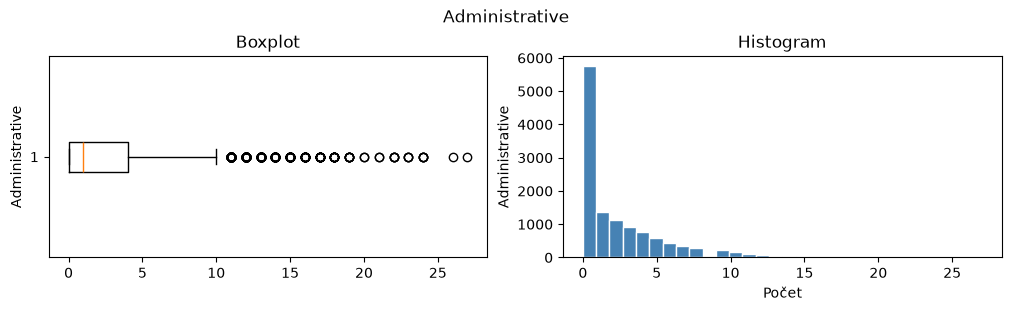
\includegraphics[width=\linewidth,height=0.78\textheight,keepaspectratio]{graf_01.png}
\end{center}

\begin{center}
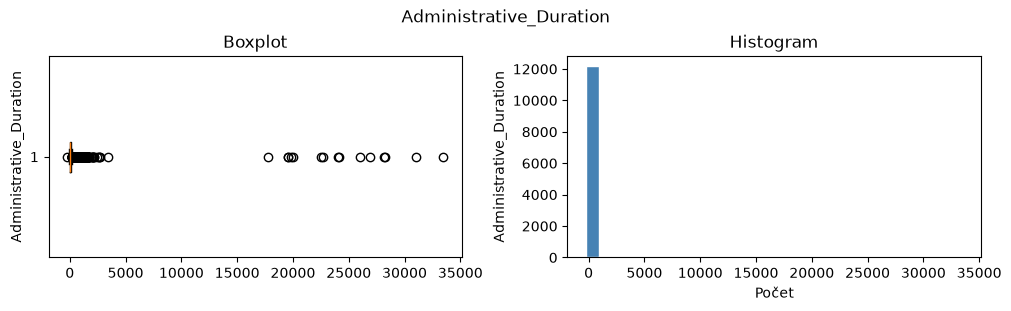
\includegraphics[width=\linewidth,height=0.78\textheight,keepaspectratio]{graf_02.png}
\end{center}

\begin{center}
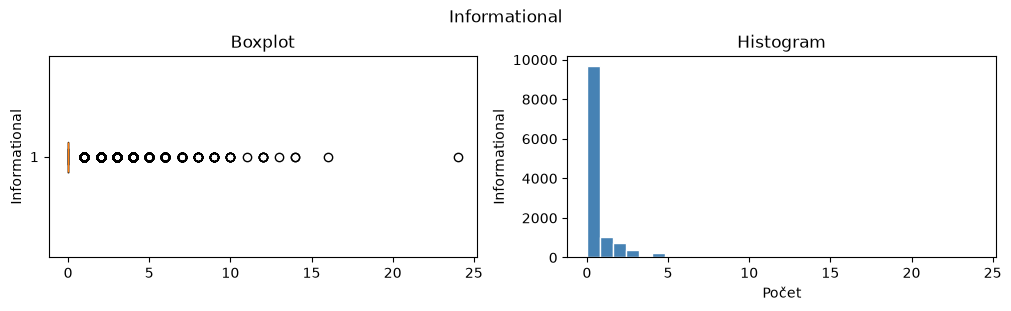
\includegraphics[width=\linewidth,height=0.78\textheight,keepaspectratio]{graf_03.png}
\end{center}

\begin{center}
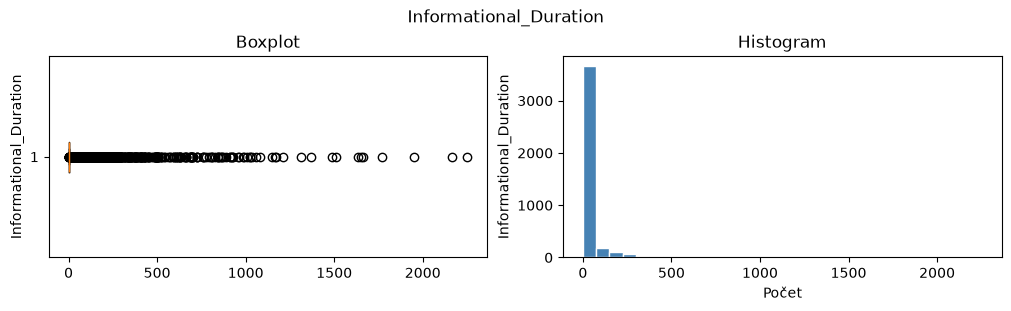
\includegraphics[width=\linewidth,height=0.78\textheight,keepaspectratio]{graf_04.png}
\end{center}

\begin{center}
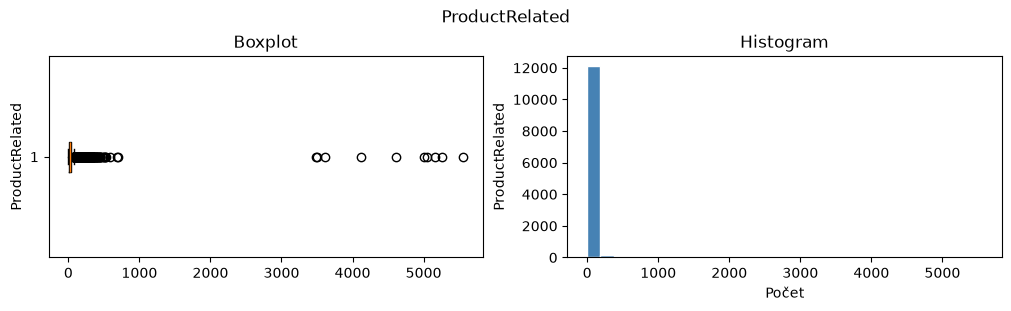
\includegraphics[width=\linewidth,height=0.78\textheight,keepaspectratio]{graf_05.png}
\end{center}

\begin{center}
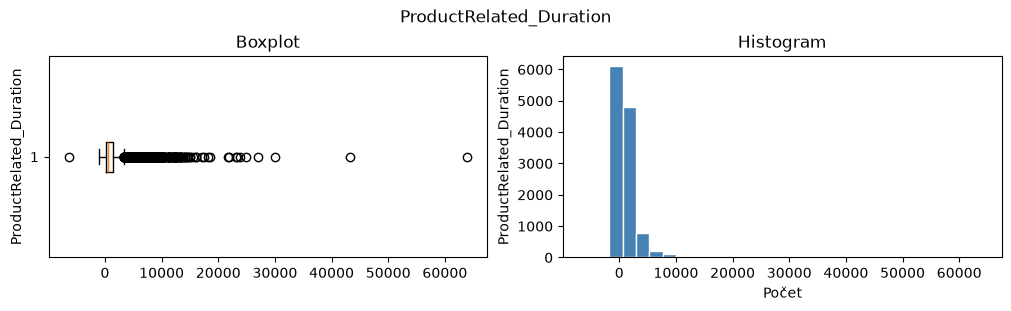
\includegraphics[width=\linewidth,height=0.78\textheight,keepaspectratio]{graf_06.png}
\end{center}

\begin{center}
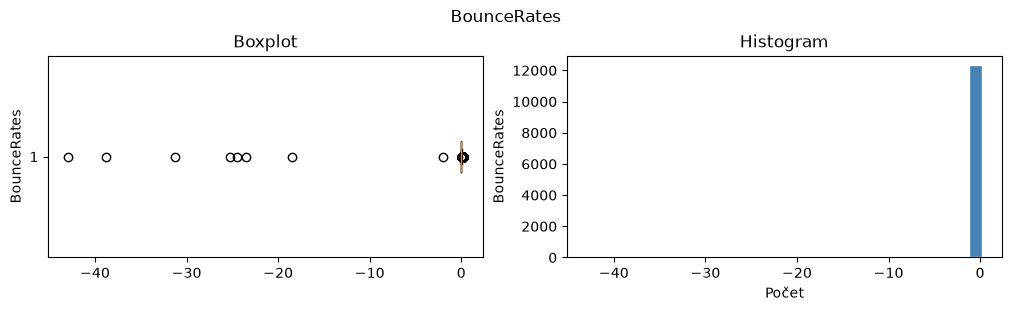
\includegraphics[width=\linewidth,height=0.78\textheight,keepaspectratio]{graf_07.png}
\end{center}

\begin{center}
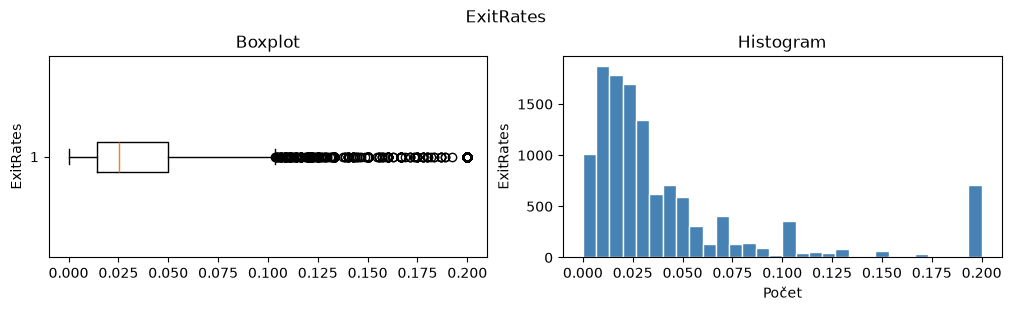
\includegraphics[width=\linewidth,height=0.78\textheight,keepaspectratio]{graf_08.png}
\end{center}

\begin{center}
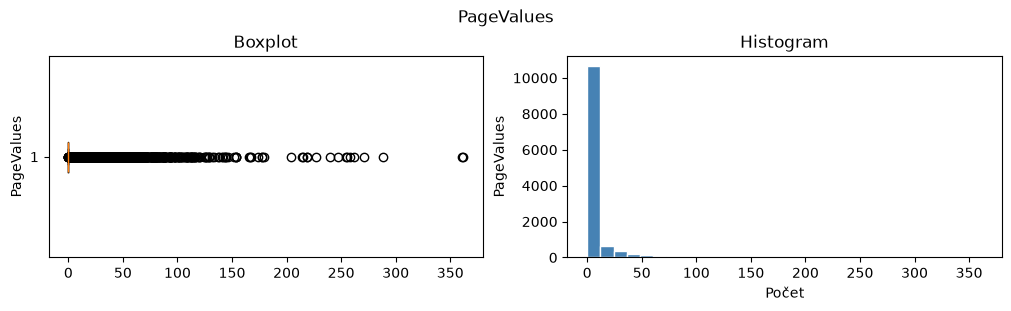
\includegraphics[width=\linewidth,height=0.78\textheight,keepaspectratio]{graf_09.png}
\end{center}

\begin{center}
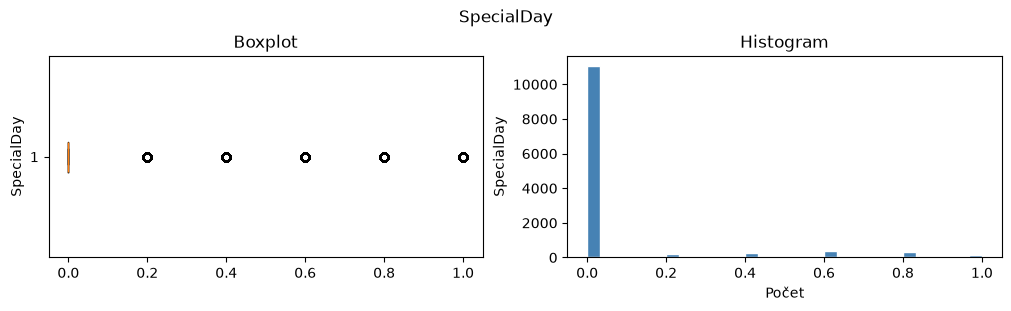
\includegraphics[width=\linewidth,height=0.78\textheight,keepaspectratio]{graf_10.png}
\end{center}

\begin{center}
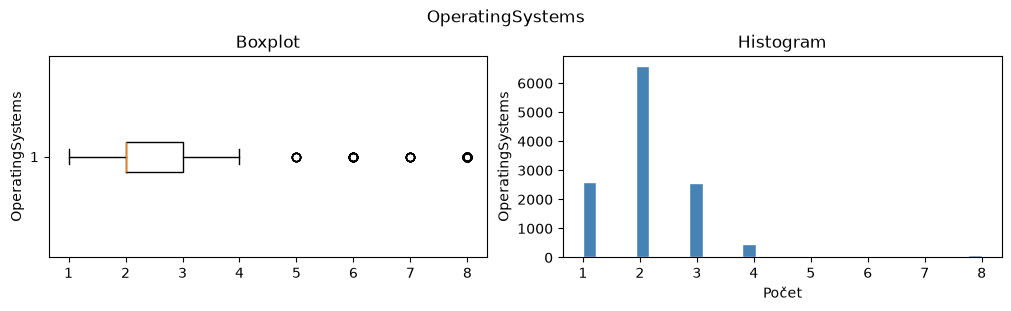
\includegraphics[width=\linewidth,height=0.78\textheight,keepaspectratio]{graf_11.png}
\end{center}

\begin{center}
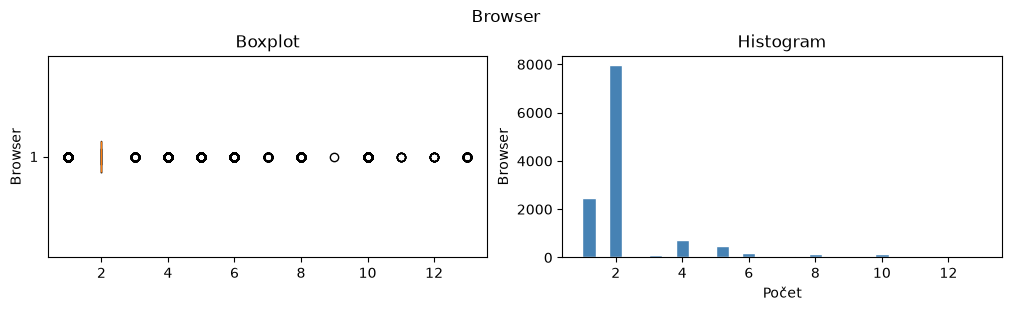
\includegraphics[width=\linewidth,height=0.78\textheight,keepaspectratio]{graf_12.png}
\end{center}

\begin{center}
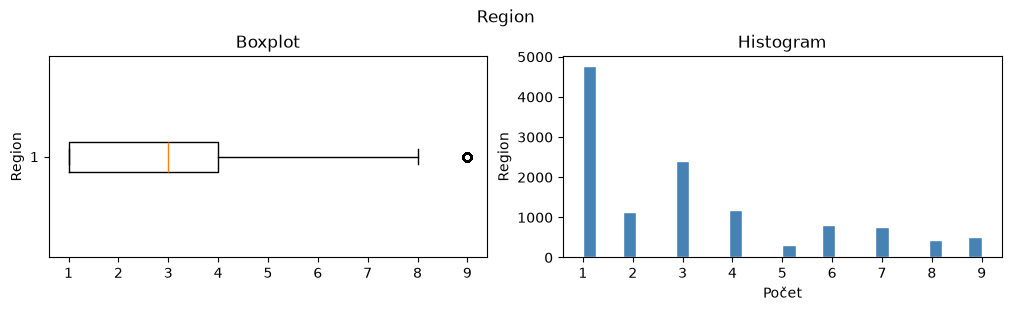
\includegraphics[width=\linewidth,height=0.78\textheight,keepaspectratio]{graf_13.png}
\end{center}

\begin{center}
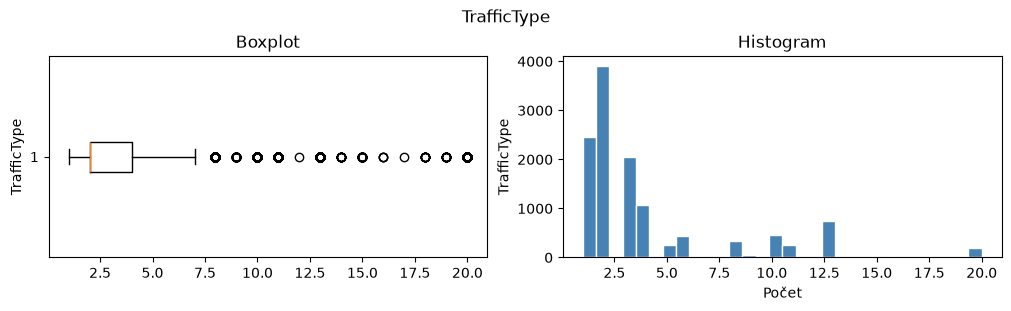
\includegraphics[width=\linewidth,height=0.78\textheight,keepaspectratio]{graf_14.png}
\end{center}

\begin{center}
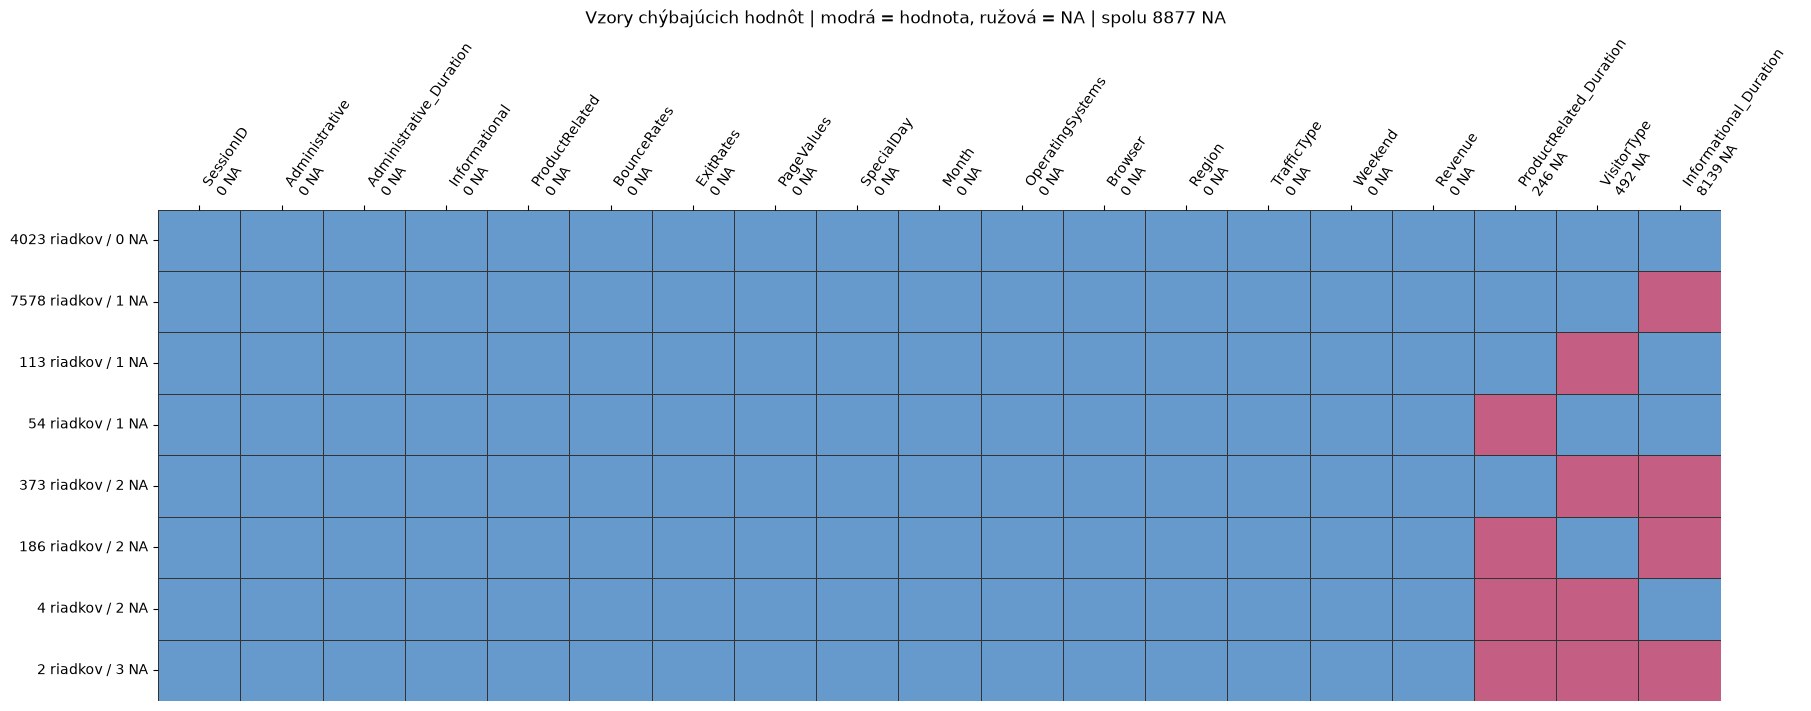
\includegraphics[width=\linewidth,height=0.78\textheight,keepaspectratio]{graf_15.png}
\end{center}

V cca 2/3 (8139/12334) dát chýba hodnota (NA) v poslednom stĺpci Informational\_\allowbreak{}Duration, čo není ani vhodné dopĺňať/nahrádzať, preto tento stĺpec je jednoduchšie a lepšie dropnúť. Riadky s chýbajúcim Product\allowbreak{}Related\_\allowbreak{}Duration a Visitor\allowbreak{}Type odstraňujem pre chýbajúce hodnotu, čo predstavuje 732 riadkov.

\begin{longtable}{>{\raggedright\arraybackslash}p{0.31000\linewidth}>{\raggedright\arraybackslash}p{0.18467\linewidth}>{\raggedright\arraybackslash}p{0.18467\linewidth}>{\raggedright\arraybackslash}p{0.18467\linewidth}}
 & count & mean & std \\
\hline
\endhead
Administrative & 11601.000000 & 2.326437 & 3.327508 \\
Administrative\_\allowbreak{}Duration & 11601.000000 & 112.502691 & 901.008974 \\
Informational & 11601.000000 & 0.507801 & 1.270743 \\
Product\allowbreak{}Related & 11601.000000 & 35.006637 & 127.664326 \\
Product\allowbreak{}Related\_\allowbreak{}Duration & 11601.000000 & 1199.481299 & 1918.490414 \\
Bounce\allowbreak{}Rates & 11601.000000 & 0.004117 & 0.748188 \\
Exit\allowbreak{}Rates & 11601.000000 & 0.042697 & 0.048397 \\
Page\allowbreak{}Values & 11601.000000 & 6.154971 & 19.006150 \\
Special\allowbreak{}Day & 11601.000000 & 0.061546 & 0.199062 \\
Operating\allowbreak{}Systems & 11601.000000 & 2.122662 & 0.910592 \\
Browser & 11601.000000 & 2.351608 & 1.708669 \\
Region & 11601.000000 & 3.140160 & 2.394896 \\
Traffic\allowbreak{}Type & 11601.000000 & 4.077752 & 4.027833 \\
\end{longtable}

\begin{longtable}{>{\raggedright\arraybackslash}p{0.31000\linewidth}>{\raggedright\arraybackslash}p{0.18467\linewidth}>{\raggedright\arraybackslash}p{0.18467\linewidth}>{\raggedright\arraybackslash}p{0.18467\linewidth}}
 & min & 25\% & 50\% \\
\hline
\endhead
Administrative & 0.000000 & 0.000000 & 1.000000 \\
Administrative\_\allowbreak{}Duration & -214.548633 & 0.000000 & 8.000000 \\
Informational & 0.000000 & 0.000000 & 0.000000 \\
Product\allowbreak{}Related & 0.000000 & 7.000000 & 18.000000 \\
Product\allowbreak{}Related\_\allowbreak{}Duration & -6423.973010 & 185.000000 & 604.000000 \\
Bounce\allowbreak{}Rates & -42.953427 & 0.000000 & 0.003014 \\
Exit\allowbreak{}Rates & 0.000000 & 0.014251 & 0.025000 \\
Page\allowbreak{}Values & 0.000000 & 0.000000 & 0.000000 \\
Special\allowbreak{}Day & 0.000000 & 0.000000 & 0.000000 \\
Operating\allowbreak{}Systems & 1.000000 & 2.000000 & 2.000000 \\
Browser & 1.000000 & 2.000000 & 2.000000 \\
Region & 1.000000 & 1.000000 & 3.000000 \\
Traffic\allowbreak{}Type & 1.000000 & 2.000000 & 2.000000 \\
\end{longtable}

\begin{longtable}{>{\raggedright\arraybackslash}p{0.31000\linewidth}>{\raggedright\arraybackslash}p{0.29400\linewidth}>{\raggedright\arraybackslash}p{0.29400\linewidth}}
 & 75\% & max \\
\hline
\endhead
Administrative & 4.000000 & 27.000000 \\
Administrative\_\allowbreak{}Duration & 94.600000 & 33466.707646 \\
Informational & 0.000000 & 24.000000 \\
Product\allowbreak{}Related & 38.000000 & 5258.000000 \\
Product\allowbreak{}Related\_\allowbreak{}Duration & 1467.654221 & 63973.522230 \\
Bounce\allowbreak{}Rates & 0.016667 & 0.200000 \\
Exit\allowbreak{}Rates & 0.050000 & 0.200000 \\
Page\allowbreak{}Values & 0.000000 & 361.763742 \\
Special\allowbreak{}Day & 0.000000 & 1.000000 \\
Operating\allowbreak{}Systems & 3.000000 & 8.000000 \\
Browser & 2.000000 & 13.000000 \\
Region & 4.000000 & 9.000000 \\
Traffic\allowbreak{}Type & 4.000000 & 20.000000 \\
\end{longtable}

\subsubsection*{removing outliers}

\begin{center}
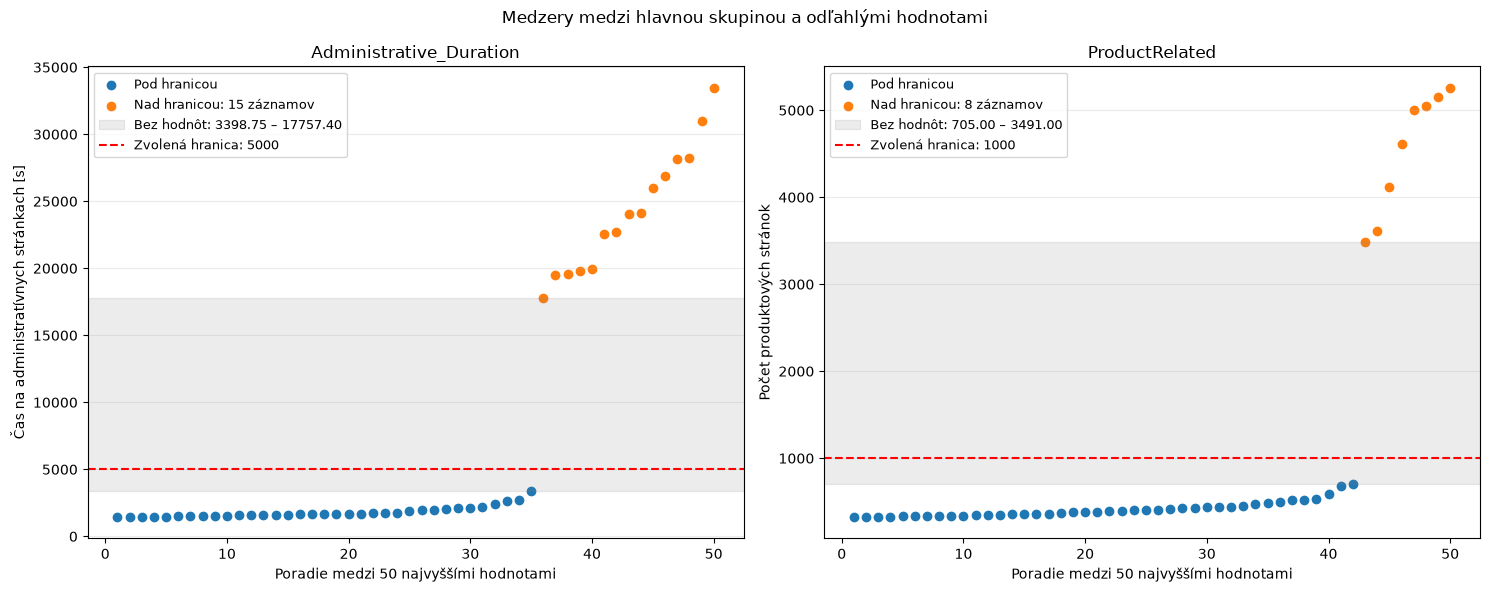
\includegraphics[width=\linewidth,height=0.78\textheight,keepaspectratio]{graf_16.png}
\end{center}

odľahlé záznamy

Počty riadkov: 11601, 11557.

Hranice 5 000s a 1 000 stránok ležia v medzerách medzi ostatnými hodnotami a dvoma odľahlými skupinami. Drop duplicates odstráni úplne identické riadky, pričom návštevy s rôznymi Session\allowbreak{}ID ponechá. Vysoké Page\allowbreak{}Values a dlhé Product\allowbreak{}Related\_\allowbreak{}Duration ponechávam, lebo samotná veľkosť hodnoty nepreukazuje chybu a môže predstavovať hodnotný nákup alebo dlhú návštevu.

Po vyčistení sa počet riadkov znížil z 11 601 na 11 557, kde sa odstráni 18 neplatných záznamov, 23 kladných outlierov a 3 duplicity.

\begin{center}
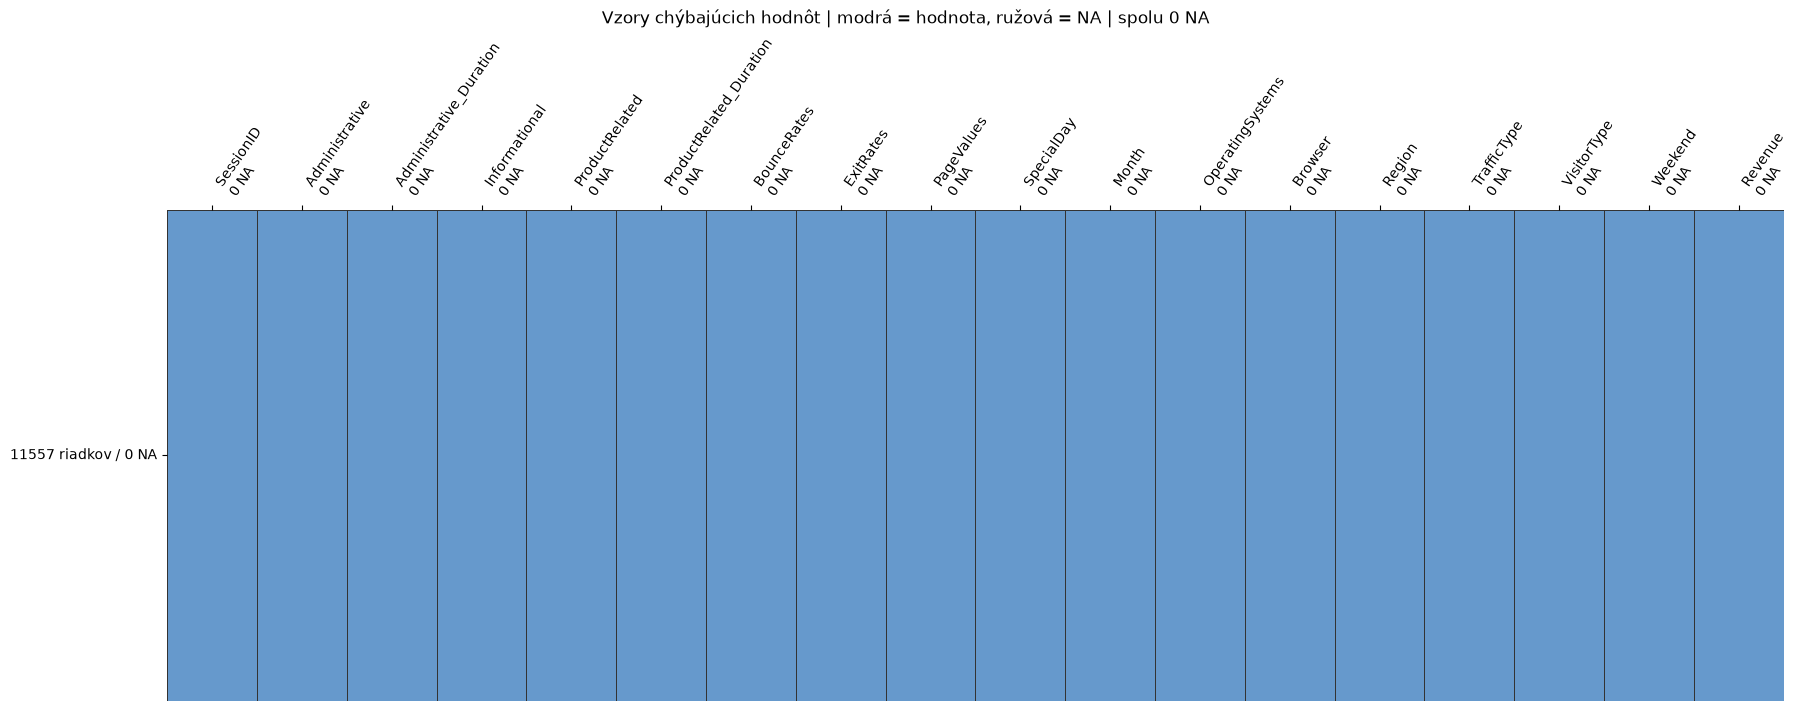
\includegraphics[width=\linewidth,height=0.78\textheight,keepaspectratio]{graf_17.png}
\end{center}

\subsection*{Visitor\allowbreak{}Type vs Product\allowbreak{}Related a Page\allowbreak{}Values}

Visitor\allowbreak{}Type

Returning\_\allowbreak{}Visitor: 9887.

New\_\allowbreak{}Visitor: 1592.

Other: 78.

Názov: count. Typ údajov: int64.

použitý log(1 + x) (log1p), kvôli normalizácii veľmi odľahlých hodnôt a obsahovaní 0 hodnôt, logaritmus 1+x zachová 0 na 0, normalizácia zachovaná aj kvôli porovnaniu rôznych skupín

\begin{center}
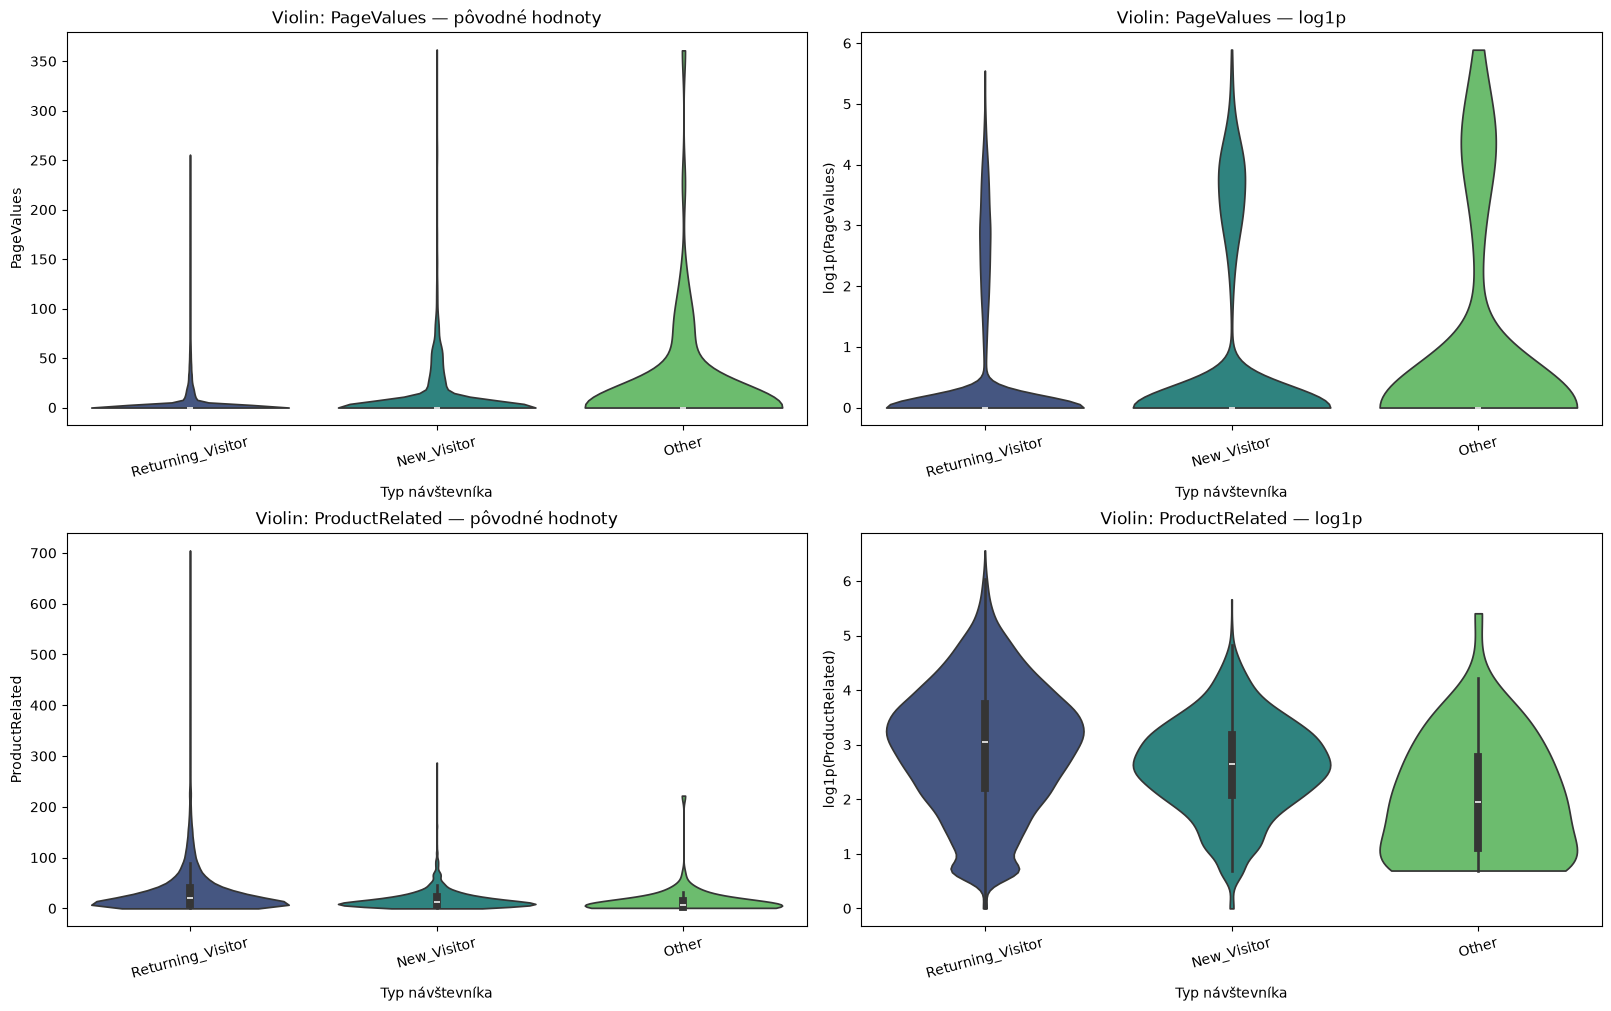
\includegraphics[width=\linewidth,height=0.78\textheight,keepaspectratio]{graf_18.png}
\end{center}

Pri Page\allowbreak{}Values sa vo všetkých skupinách väčšina hodnôt sústreďuje pri nule. Rozdelenia majú dlhé chvosty, kde sa ťahajú k vysokým hodnotám. Transformácia log1p zlepšuje zobrazenie hodnôt, kde je vidno že v skupine Other je hustota posunutá k vyšším hodnotám než pri vracajúcich sa návštevníkov.

Pri Product\allowbreak{}Related pôvodnú mierku výrazne ovplyvňujú extrémne hodnoty vracajúcich sa návštevníkov. Po transformácii sú rozdiely čitateľnejšie, kde vracajúci sa návštevníci majú najvyšší medián a najnižší ostatný typ návštevníkov. Vracajúci návštevníci navštevujú viac produktovo súvisiacich stránok.

\begin{center}
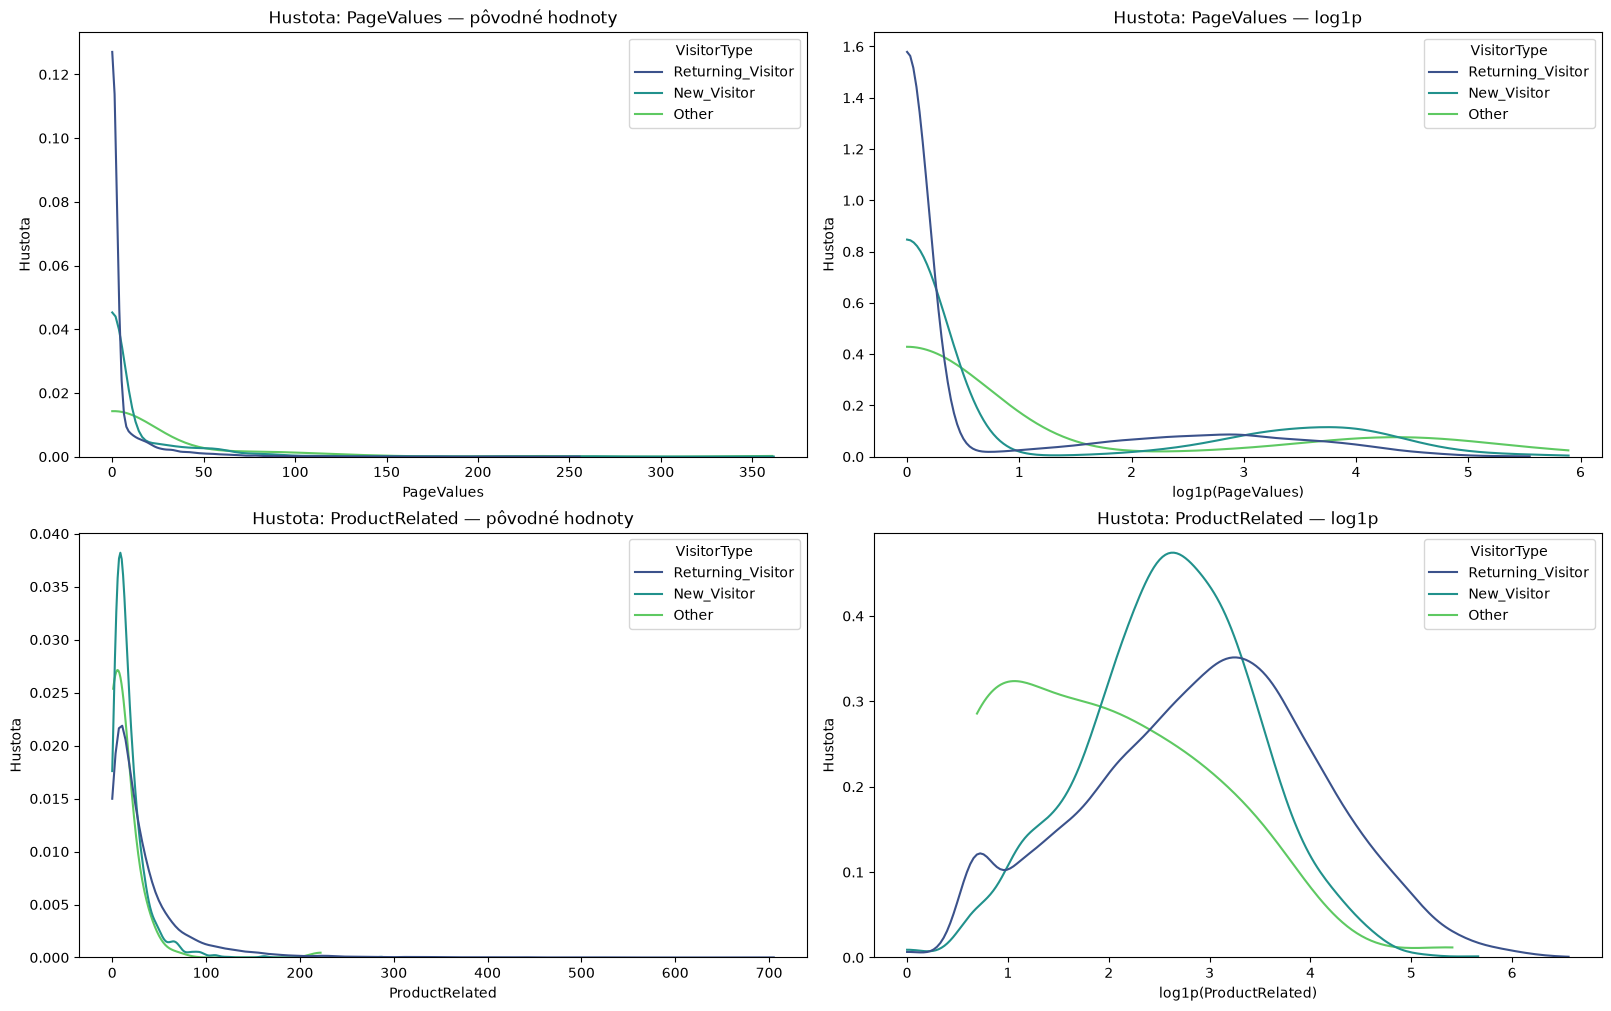
\includegraphics[width=\linewidth,height=0.78\textheight,keepaspectratio]{graf_19.png}
\end{center}

Pri Page\allowbreak{}Values vidíme výrazný vrchol pri nule a dlhý chvost pri všetkých skupinách. Pri nule je najhustejšia skupina vracajúcich sa zákazníkov, pri skupinách New\_\allowbreak{}Visitor a Other sú hodnoty širšie.

Pri Product\allowbreak{}Related je najvyššia hodnota v skupine nových zákazníkov v oblasti medzi 2 a 4 (os logaritmu skupiny). Skupina Other má najhustejšiu hodnotu bližšie k nule a vracajúci sa zákazníci majú najhustejšiu hodnotu vo vyšších hodnotách.

\subsection*{Month (mesiac poslednej návštevy) a Revenue}

Porovnávam podiel sessionov ukončených nákupom v jednotlivých mesiacoch. Počet nákupov / počet sessions v danom mesiaci. Mesačné podiely a chybové úsečky, v ich 95\% Wilson intervaloch spoľahlivosti, čo vyjadruje neistotu odhadu pri predpoklade nezávislých sessionov. V datasete chýbajú dáta za mesiac január a apríl.

Boxplot sumarizuje rozdelenie mesačných podielov.

\begin{center}
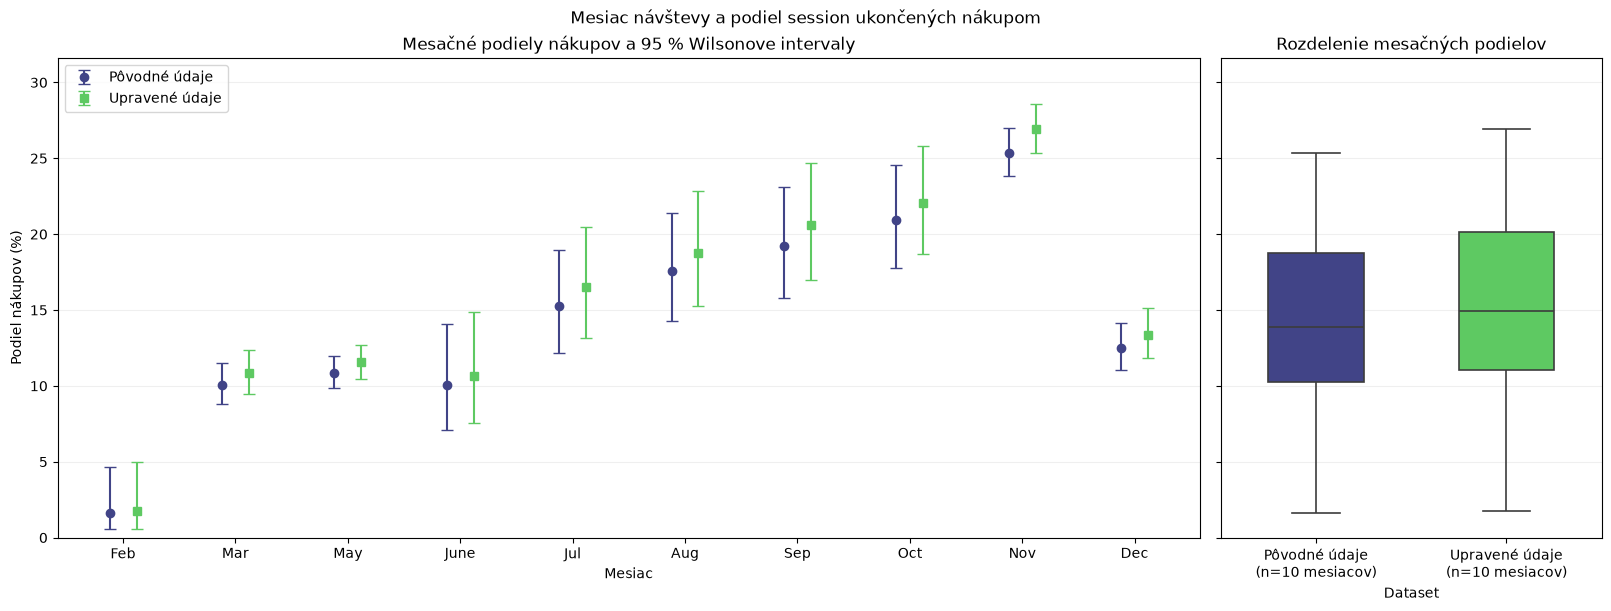
\includegraphics[width=\linewidth,height=0.78\textheight,keepaspectratio]{graf_20.png}
\end{center}

\begin{longtable}{>{\raggedright\arraybackslash}p{0.31000\linewidth}>{\raggedright\arraybackslash}p{0.18467\linewidth}>{\raggedright\arraybackslash}p{0.18467\linewidth}>{\raggedright\arraybackslash}p{0.18467\linewidth}}
Month & Feb & Mar & May \\
\hline
\endhead
Pôvodné údaje / sessions & 185 & 1907 & 3365 \\
Pôvodné údaje / purchases & 3 & 192 & 365 \\
Pôvodné údaje / purchase\_\allowbreak{}rate & 1.62 & 10.07 & 10.85 \\
Pôvodné údaje / ci\_\allowbreak{}lower & 0.55 & 8.80 & 9.84 \\
Pôvodné údaje / ci\_\allowbreak{}upper & 4.66 & 11.50 & 11.94 \\
Upravené údaje / sessions & 173 & 1771 & 3161 \\
Upravené údaje / purchases & 3 & 192 & 365 \\
Upravené údaje / purchase\_\allowbreak{}rate & 1.73 & 10.84 & 11.55 \\
Upravené údaje / ci\_\allowbreak{}lower & 0.59 & 9.48 & 10.48 \\
Upravené údaje / ci\_\allowbreak{}upper & 4.97 & 12.37 & 12.71 \\
\end{longtable}

\begin{longtable}{>{\raggedright\arraybackslash}p{0.31000\linewidth}>{\raggedright\arraybackslash}p{0.18467\linewidth}>{\raggedright\arraybackslash}p{0.18467\linewidth}>{\raggedright\arraybackslash}p{0.18467\linewidth}}
Month & June & Jul & Aug \\
\hline
\endhead
Pôvodné údaje / sessions & 288 & 432 & 433 \\
Pôvodné údaje / purchases & 29 & 66 & 76 \\
Pôvodné údaje / purchase\_\allowbreak{}rate & 10.07 & 15.28 & 17.55 \\
Pôvodné údaje / ci\_\allowbreak{}lower & 7.10 & 12.19 & 14.26 \\
Pôvodné údaje / ci\_\allowbreak{}upper & 14.09 & 18.98 & 21.42 \\
Upravené údaje / sessions & 272 & 400 & 405 \\
Upravené údaje / purchases & 29 & 66 & 76 \\
Upravené údaje / purchase\_\allowbreak{}rate & 10.66 & 16.50 & 18.77 \\
Upravené údaje / ci\_\allowbreak{}lower & 7.53 & 13.18 & 15.26 \\
Upravené údaje / ci\_\allowbreak{}upper & 14.89 & 20.45 & 22.85 \\
\end{longtable}

\begin{longtable}{>{\raggedright\arraybackslash}p{0.31000\linewidth}>{\raggedright\arraybackslash}p{0.18467\linewidth}>{\raggedright\arraybackslash}p{0.18467\linewidth}>{\raggedright\arraybackslash}p{0.18467\linewidth}}
Month & Sep & Oct & Nov \\
\hline
\endhead
Pôvodné údaje / sessions & 448 & 549 & 2999 \\
Pôvodné údaje / purchases & 86 & 115 & 761 \\
Pôvodné údaje / purchase\_\allowbreak{}rate & 19.20 & 20.95 & 25.38 \\
Pôvodné údaje / ci\_\allowbreak{}lower & 15.82 & 17.75 & 23.85 \\
Pôvodné údaje / ci\_\allowbreak{}upper & 23.10 & 24.55 & 26.96 \\
Upravené údaje / sessions & 418 & 522 & 2821 \\
Upravené údaje / purchases & 86 & 115 & 760 \\
Upravené údaje / purchase\_\allowbreak{}rate & 20.57 & 22.03 & 26.94 \\
Upravené údaje / ci\_\allowbreak{}lower & 16.98 & 18.69 & 25.34 \\
Upravené údaje / ci\_\allowbreak{}upper & 24.71 & 25.78 & 28.61 \\
\end{longtable}

\begin{longtable}{>{\raggedright\arraybackslash}p{0.31000\linewidth}>{\raggedright\arraybackslash}p{0.62200\linewidth}}
Month & Dec \\
\hline
\endhead
Pôvodné údaje / sessions & 1727 \\
Pôvodné údaje / purchases & 216 \\
Pôvodné údaje / purchase\_\allowbreak{}rate & 12.51 \\
Pôvodné údaje / ci\_\allowbreak{}lower & 11.03 \\
Pôvodné údaje / ci\_\allowbreak{}upper & 14.15 \\
Upravené údaje / sessions & 1614 \\
Upravené údaje / purchases & 216 \\
Upravené údaje / purchase\_\allowbreak{}rate & 13.38 \\
Upravené údaje / ci\_\allowbreak{}lower & 11.81 \\
Upravené údaje / ci\_\allowbreak{}upper & 15.13 \\
\end{longtable}

Najvyšší podiel nákupov je za mesiac november, približne 25.4\% v neupravených a v upravených 26.9\% dátach. Najnižšie je za mesiac február, kde dosahuje podiel iba 1.6\% a 1.7\%.

Intervaly spoľahlivosti spresňujú informáciu o presnosti odhadov, kde závisí od počtu sessions aj od podielu nákupov. Máj má užší interval ako mesiac august, ktorý obsahuje menej sessionov.

Pri čistení boli odstránené iba sessiony bez nákupu, počet nákupov preto ostal rovnaký, zatiaľ čo sessiony klesli, čo zvýšilo podiel nákupov v upravených dátach.

\subsubsection*{Correlation of session and purchase by month}

\begin{center}
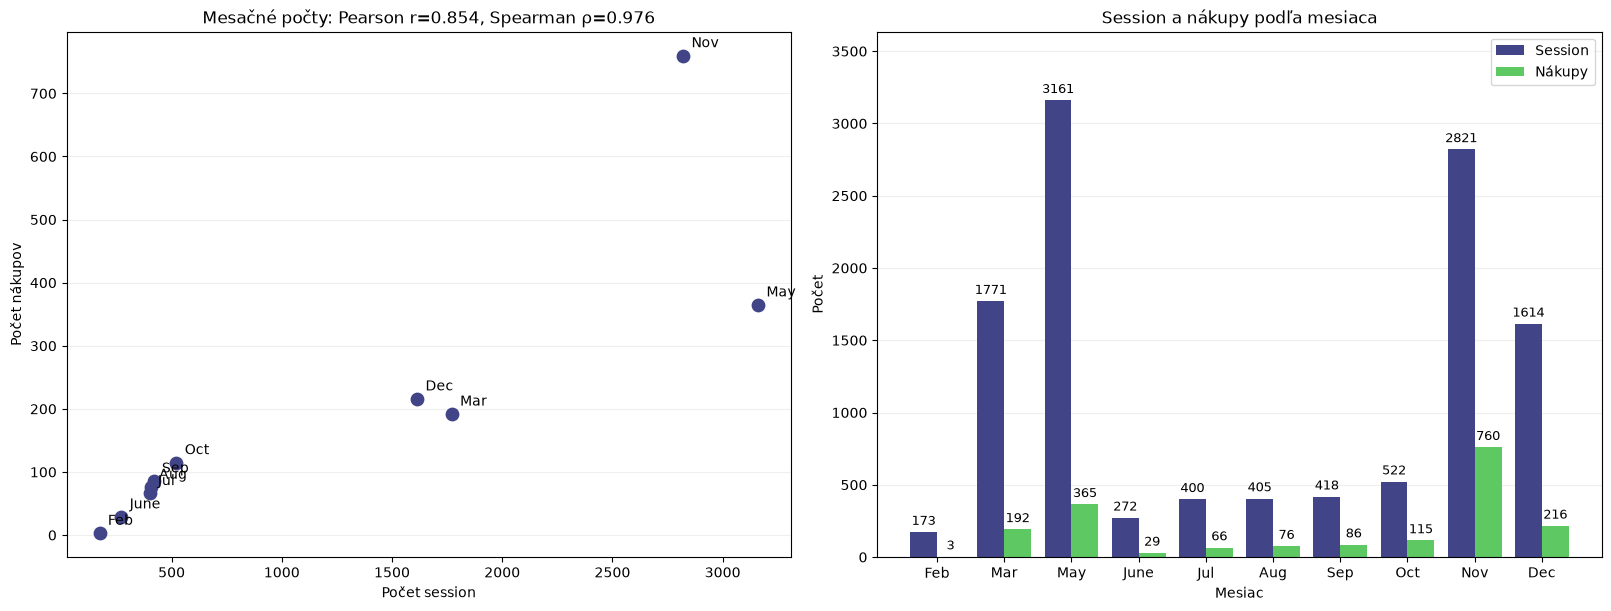
\includegraphics[width=\linewidth,height=0.78\textheight,keepaspectratio]{graf_21.png}
\end{center}

\begin{longtable}{>{\raggedright\arraybackslash}p{0.31000\linewidth}>{\raggedright\arraybackslash}p{0.18467\linewidth}>{\raggedright\arraybackslash}p{0.18467\linewidth}>{\raggedright\arraybackslash}p{0.18467\linewidth}}
Mesiac & Počet session & Počet nákupov & Podiel nákupov (\%) \\
\hline
\endhead
Feb & 173 & 3 & 1.73 \\
Mar & 1771 & 192 & 10.84 \\
May & 3161 & 365 & 11.55 \\
June & 272 & 29 & 10.66 \\
Jul & 400 & 66 & 16.50 \\
Aug & 405 & 76 & 18.77 \\
Sep & 418 & 86 & 20.57 \\
Oct & 522 & 115 & 22.03 \\
Nov & 2821 & 760 & 26.94 \\
Dec & 1614 & 216 & 13.38 \\
Spolu / priemerný podiel / korelácie medzi mesiacmi & 11557 & 1908 & 15.30 \\
\end{longtable}

\begin{longtable}{>{\raggedright\arraybackslash}p{0.31000\linewidth}>{\raggedright\arraybackslash}p{0.29400\linewidth}>{\raggedright\arraybackslash}p{0.29400\linewidth}}
Mesiac & Pearson & Spearman \\
\hline
\endhead
Feb & — & — \\
Mar & — & — \\
May & — & — \\
June & — & — \\
Jul & — & — \\
Aug & — & — \\
Sep & — & — \\
Oct & — & — \\
Nov & — & — \\
Dec & — & — \\
Spolu / priemerný podiel / korelácie medzi mesiacmi & 0.854 & 0.976 \\
\end{longtable}

Pearsonova korelácia r = 0.853 naznačuje silný lineárny vzťah. Spearmanova korelácia \ensuremath{\rho} = 0.976 ukazuje, že mesiace s vyššou návštevnosťou majú takmer vždy aj vyšší počet nákupov.

Máj mal najviac sessionov 3 171 ale nákupom skončilo 365, podiel 11.5\%. November mal menej sessionov 2 826 no najviac nákupov 756, čo je aj najvyšší podiel nákupov 26.9\%. Najnižší podiel dosiahol za mesiac február a to 1.7\%.

\subsection*{Product\allowbreak{}Related a Exit\allowbreak{}Rates}

Hexbin graf ukazuje počet produktových stránok oproti priemernej miere odchodu zo stránok navštívených v sessions. Používam log1p, čo zachová nuly a zlepšuje čitateľnosť veľkého rozsahu. Farba vyjadruje počet sessionov v hexagóne.

\begin{center}
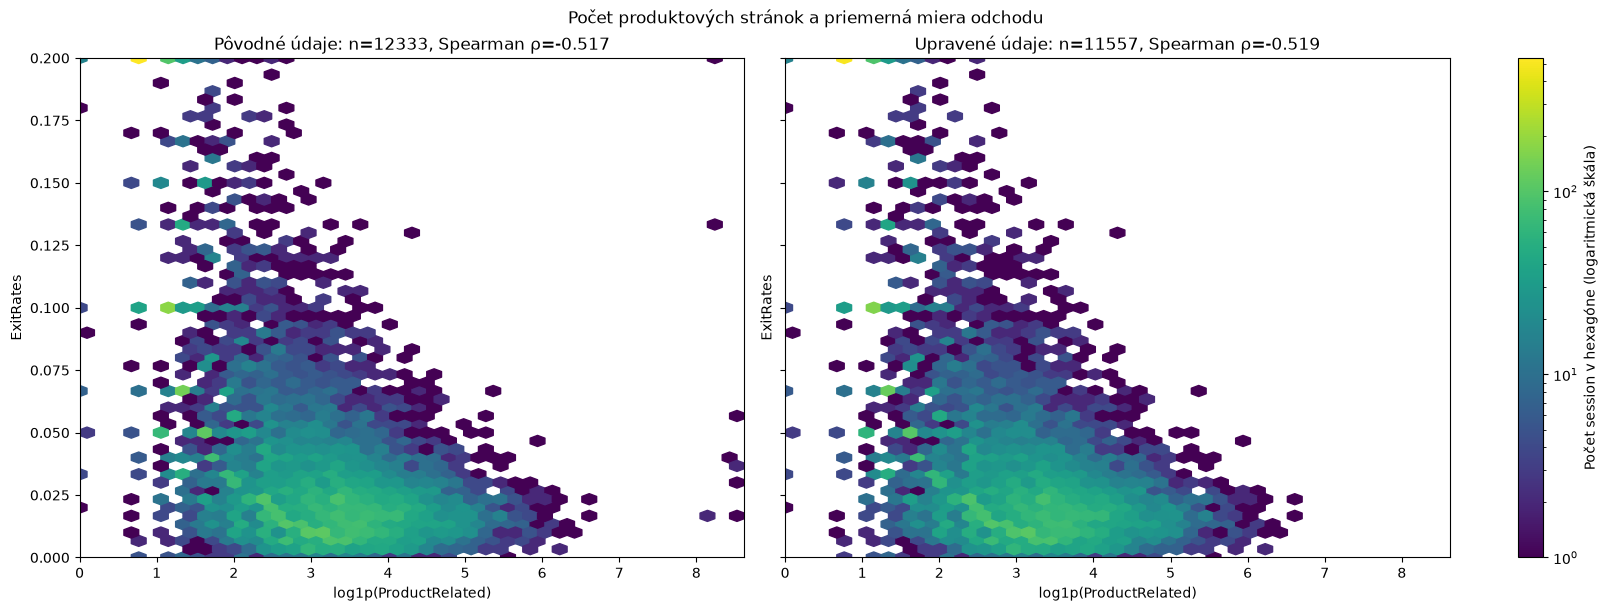
\includegraphics[width=\linewidth,height=0.78\textheight,keepaspectratio]{graf_22.png}
\end{center}

\begin{longtable}{>{\raggedright\arraybackslash}p{0.31000\linewidth}>{\raggedright\arraybackslash}p{0.18467\linewidth}>{\raggedright\arraybackslash}p{0.18467\linewidth}>{\raggedright\arraybackslash}p{0.18467\linewidth}}
Dataset & Počet session & Spearman & Medián Exit\allowbreak{}Rates (0–1 produktových stránok) \\
\hline
\endhead
Pôvodné údaje & 12333 & -0.517 & 0.2 \\
Upravené údaje & 11557 & -0.519 & 0.2 \\
\end{longtable}

\begin{longtable}{>{\raggedright\arraybackslash}p{0.31000\linewidth}>{\raggedright\arraybackslash}p{0.62200\linewidth}}
Dataset & Medián Exit\allowbreak{}Rates (\textgreater{}50 produktových stránok) \\
\hline
\endhead
Pôvodné údaje & 0.017 \\
Upravené údaje & 0.017 \\
\end{longtable}

S rastúcim počtom navštívených produktových stránok má priemerná miera odchodu sa znižovať. Vzťah ostáva podobný pred aj po čistení, kde to naznačuje Spearmanova korelácia, ktorá je približne -0.52. Nepreukazuje sa, že viac produktových stránok priamo spôsobuje nižšiu mieru odchodu. Medián pre Exit\allowbreak{}Rates pri 0-1 produktových stránkach je 0.2 ale 0.017 pri viac ako 50 produktových stránkach.

\subsection*{Correlation of Product\allowbreak{}Related and time on them}

Počet session: 11557 | Pearson r = 0.861 | Spearman \ensuremath{\rho} = 0.884

\begin{center}
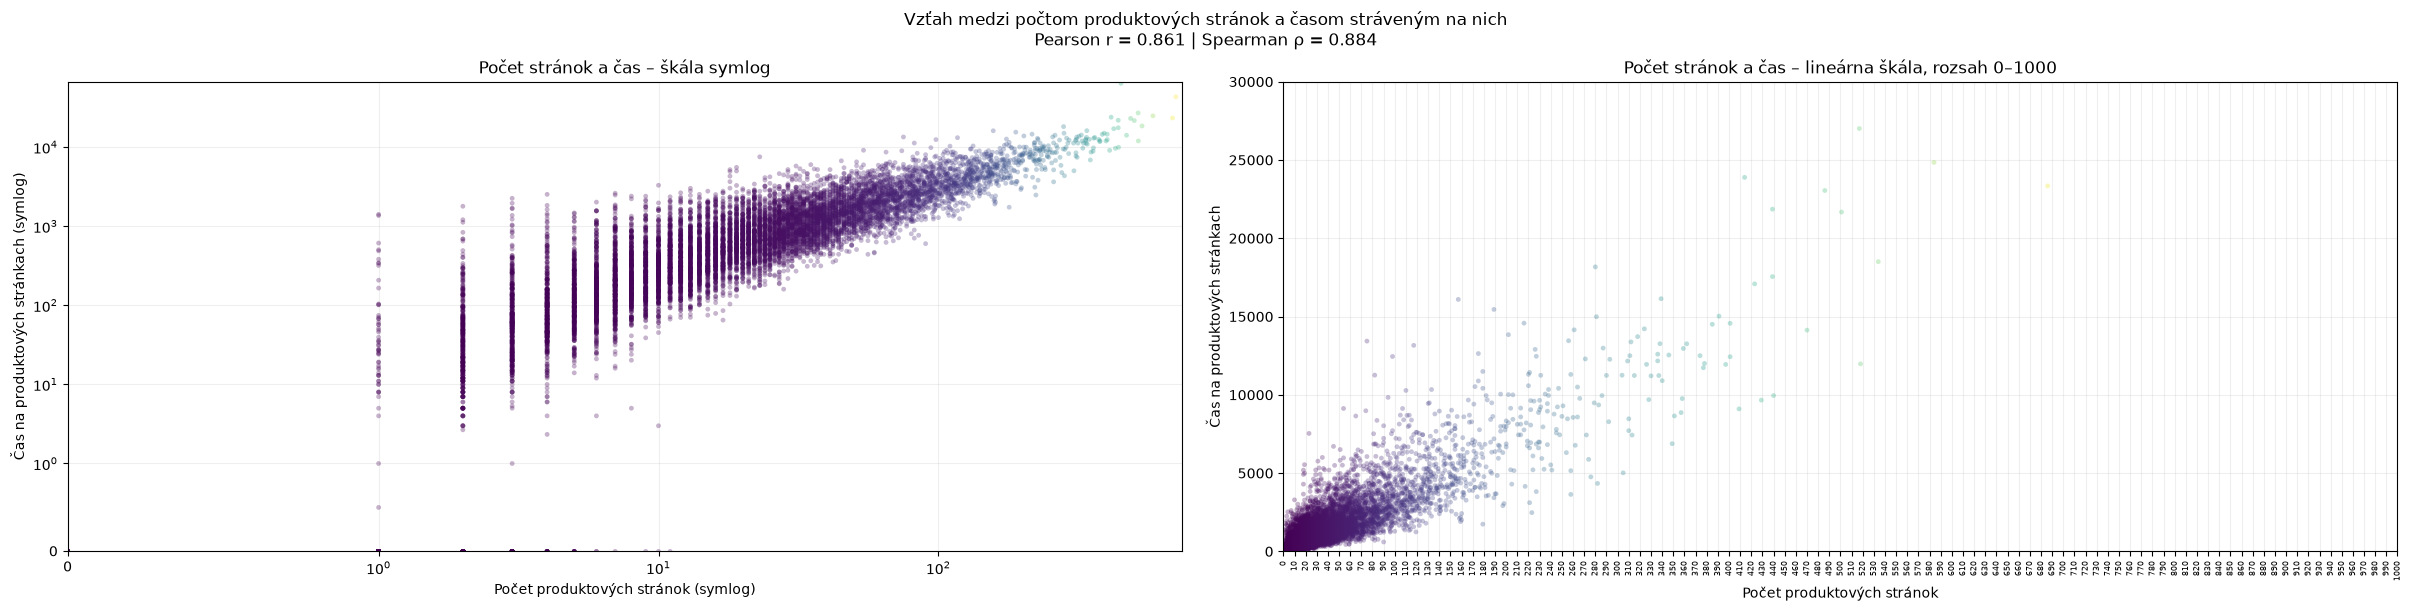
\includegraphics[width=\linewidth,height=0.78\textheight,keepaspectratio]{graf_23.png}
\end{center}

Počet session s časom nad 30 000: 2

\begin{longtable}{>{\raggedright\arraybackslash}p{0.31000\linewidth}>{\raggedright\arraybackslash}p{0.18467\linewidth}>{\raggedright\arraybackslash}p{0.18467\linewidth}>{\raggedright\arraybackslash}p{0.18467\linewidth}}
 & Session\allowbreak{}ID & Product\allowbreak{}Related & Product\allowbreak{}Related\_\allowbreak{}Duration \\
\hline
\endhead
0 & S-108071 & 449.0 & 63973.52223 \\
1 & S-105152 & 705.0 & 43171.23338 \\
\end{longtable}

Graf ukazuje, že s rastúcim počtom navštívených produktových stránok rastie aj čas strávený na nich. Pearsonova korelácia je 0.304, čo naznačuje slabšiu lineárnu závislosť. Spearmanova korelácia 0.883 ukazuje silný vzťah, vyššiemu počtu stránok väčšinou pripadá dlhší čas, hoci tento rast nie je rovnomerný.

Graf so škálou symlog umožňuje ukázať extrémne hodnoty a lepšie odhaľuje rastúci trend. Lineárny graf ukazuje, že väčšina sessionov sa sústreďuje pri nižších počtoch stránok a kratšom čase.

Pri rovnakom počte stránok sa čas medzi sessionami výrazne líši. Viditeľné sú aj extrémne hodnoty s vysokým počtom stránok a pomerne krátkym časom, ktoré môžu ovplyvňovať Pearsonovu koreláciu. Počet produktových stránok súvisí s časom návštevy, ale sám nestačí na jeho presný odhad.

\section*{Classification}

\subsection*{data separation}

Rozmery vstupov: 11557 riadkov a 16 stĺpcov.

Rozmery cieľa: 11557 hodnôt.

Kategorické stĺpce: Month, Visitor\allowbreak{}Type, Operating\allowbreak{}Systems, Browser, Region, Traffic\allowbreak{}Type.

Binárne stĺpce: Weekend.

Revenue

0: 0.834905.

1: 0.165095.

Názov: proportion. Typ údajov: float64.

\subsection*{train, val, test split}

Počty vzoriek: train 8089, val 1734, test 1734.

Rozdelenie dát na trénovacie, testovacie a validačné, kde využijem aj stratify na zachovanie pomeru voči Revenue (zachovanie tak istého pomeru nákupu v train, val a test množine). Počty sa môžu mierne líšiť od pomerov pre zaokrúhlenie na celé riadky.

\subsection*{encoding discrete cols}

One-Hot encoder vytvorí samostatné binárne stĺpce pre každú kategóriu, čo je vhodné pre diskrétne dáta (kategorické). Nezachováva vzťah, závislosť, poradie ani vzdialenosť od ostatných kategórií - mali by byť nezávislé, ale nezaručuje sa to. handle unknown umožní spracovať aj kategóriu, ktorá sa v tréningu nevyskytla a imputer doplní prípadne chýbajúce hodnoty najčastejšou kategóriou, ktorá sa vyskytla v tréningu.

\subsection*{scaling}

Standard\allowbreak{}Scaler škáluje číselné vlastnosti na približne nulový priemer a jednotkový rozptyl (napríklad aby sa čas v sekundách neprevažoval nad mierami odchodu pri fitovaní logistickej regresii). Diskrétne stĺpce ponechávam v 0/1, prípadne chýbajúce hodnoty sa doplnia modusom.

Všetko je organizované v Pipeline, aby sa kódovanie, škálovanie, imputácia využívalo pri každom folde trénovania.

\subsection*{modely}

Random\allowbreak{}Forest: 64 kombinácií

Logistic\allowbreak{}Regression: 12 kombinácií

Decision\allowbreak{}Tree: 10 kombinácií

\subsection*{Grid\allowbreak{}Search\allowbreak{}CV}

Pri cross-validation sa vyberajú parametre podľa priemernej accuracy v 5 stratified k-folds tréningovej množiny.

\subsection*{experiments, fit and eval}

\subsubsection*{fit}

Rozdelenie 70/15/15 | Random\allowbreak{}Forest

Počet foldov: 1. Počet kandidátov: 64. Celkový počet trénovaní: 64.

Najlepšie parametre Grid\allowbreak{}Search\allowbreak{}CV: maximálna hĺbka 15, počet zvažovaných vlastností 10, minimálny počet vzoriek v liste 3.

Najlepšie skóre Grid\allowbreak{}Search\allowbreak{}CV: 0.8967704728950404.

Rozdelenie 70/15/15 | Logistic\allowbreak{}Regression

Počet foldov: 1. Počet kandidátov: 12. Celkový počet trénovaní: 12.

Najlepšie parametre Grid\allowbreak{}Search\allowbreak{}CV: parameter C 0.1 (typ float64), váženie tried žiadne.

Najlepšie skóre Grid\allowbreak{}Search\allowbreak{}CV: 0.8748558246828143.

Rozdelenie 70/15/15 | Decision\allowbreak{}Tree

Počet foldov: 1. Počet kandidátov: 10. Celkový počet trénovaní: 10.

Najlepšie parametre Grid\allowbreak{}Search\allowbreak{}CV: maximálna hĺbka 5, minimálny počet vzoriek v liste 1.

Najlepšie skóre Grid\allowbreak{}Search\allowbreak{}CV: 0.8927335640138409.

Rozdelenie 80/10/10 | Random\allowbreak{}Forest

Počet foldov: 1. Počet kandidátov: 64. Celkový počet trénovaní: 64.

Najlepšie parametre Grid\allowbreak{}Search\allowbreak{}CV: maximálna hĺbka 15, počet zvažovaných vlastností 13, minimálny počet vzoriek v liste 3.

Najlepšie skóre Grid\allowbreak{}Search\allowbreak{}CV: 0.8987889273356401.

Rozdelenie 80/10/10 | Logistic\allowbreak{}Regression

Počet foldov: 1. Počet kandidátov: 12. Celkový počet trénovaní: 12.

Najlepšie parametre Grid\allowbreak{}Search\allowbreak{}CV: parameter C 0.1 (typ float64), váženie tried žiadne.

Najlepšie skóre Grid\allowbreak{}Search\allowbreak{}CV: 0.879757785467128.

Rozdelenie 80/10/10 | Decision\allowbreak{}Tree

Počet foldov: 1. Počet kandidátov: 10. Celkový počet trénovaní: 10.

Najlepšie parametre Grid\allowbreak{}Search\allowbreak{}CV: maximálna hĺbka 3, minimálny počet vzoriek v liste 1.

Najlepšie skóre Grid\allowbreak{}Search\allowbreak{}CV: 0.8875432525951558.

Rozdelenie 70/10/20 | Random\allowbreak{}Forest

Počet foldov: 1. Počet kandidátov: 64. Celkový počet trénovaní: 64.

Najlepšie parametre Grid\allowbreak{}Search\allowbreak{}CV: maximálna hĺbka 10, počet zvažovaných vlastností 13, minimálny počet vzoriek v liste 1.

Najlepšie skóre Grid\allowbreak{}Search\allowbreak{}CV: 0.9117647058823529.

Rozdelenie 70/10/20 | Logistic\allowbreak{}Regression

Počet foldov: 1. Počet kandidátov: 12. Celkový počet trénovaní: 12.

Najlepšie parametre Grid\allowbreak{}Search\allowbreak{}CV: parameter C 1.0 (typ float64), váženie tried žiadne.

Najlepšie skóre Grid\allowbreak{}Search\allowbreak{}CV: 0.8780276816608996.

Rozdelenie 70/10/20 | Decision\allowbreak{}Tree

Počet foldov: 1. Počet kandidátov: 10. Celkový počet trénovaní: 10.

Najlepšie parametre Grid\allowbreak{}Search\allowbreak{}CV: maximálna hĺbka 3, minimálny počet vzoriek v liste 1.

Najlepšie skóre Grid\allowbreak{}Search\allowbreak{}CV: 0.9013840830449827.

Rozdelenie 60/10/30 | Random\allowbreak{}Forest

Počet foldov: 1. Počet kandidátov: 64. Celkový počet trénovaní: 64.

Najlepšie parametre Grid\allowbreak{}Search\allowbreak{}CV: maximálna hĺbka 10, počet zvažovaných vlastností 10, minimálny počet vzoriek v liste 3.

Najlepšie skóre Grid\allowbreak{}Search\allowbreak{}CV: 0.8996539792387543.

Rozdelenie 60/10/30 | Logistic\allowbreak{}Regression

Počet foldov: 1. Počet kandidátov: 12. Celkový počet trénovaní: 12.

Najlepšie parametre Grid\allowbreak{}Search\allowbreak{}CV: parameter C 0.1 (typ float64), váženie tried žiadne.

Najlepšie skóre Grid\allowbreak{}Search\allowbreak{}CV: 0.8719723183391004.

Rozdelenie 60/10/30 | Decision\allowbreak{}Tree

Počet foldov: 1. Počet kandidátov: 10. Celkový počet trénovaní: 10.

Najlepšie parametre Grid\allowbreak{}Search\allowbreak{}CV: maximálna hĺbka 5, minimálny počet vzoriek v liste 5.

Najlepšie skóre Grid\allowbreak{}Search\allowbreak{}CV: 0.8953287197231834.

\begin{longtable}{>{\raggedright\arraybackslash}p{0.31000\linewidth}>{\raggedright\arraybackslash}p{0.18467\linewidth}>{\raggedright\arraybackslash}p{0.18467\linewidth}>{\raggedright\arraybackslash}p{0.18467\linewidth}}
 & 0 & 1 & 2 \\
\hline
\endhead
Rozdelenie & 70/15/15 & 70/15/15 & 70/15/15 \\
Model & Random\allowbreak{}Forest & Logistic\allowbreak{}Regression & Decision\allowbreak{}Tree \\
Train n & 8089 & 8089 & 8089 \\
Val n & 1734 & 1734 & 1734 \\
Test n & 1734 & 1734 & 1734 \\
Train accuracy & 0.9498 & 0.8795 & 0.9119 \\
Val accuracy & 0.8968 & 0.8749 & 0.8927 \\
Grid accuracy & 0.8968 & 0.8749 & 0.8927 \\
Grid std & 0.0 & 0.0 & 0.0 \\
Test accuracy & 0.8899 & 0.8760 & 0.8795 \\
Test balanced accuracy & 0.7404 & 0.6634 & 0.7146 \\
Test F1 & 0.6078 & 0.4794 & 0.5618 \\
Test recall & 0.5175 & 0.3462 & 0.4685 \\
Baseline test accuracy & 0.8351 & 0.8351 & 0.8351 \\
Train-test rozdiel & 0.0600 & 0.0035 & 0.0324 \\
\end{longtable}

\begin{longtable}{>{\raggedright\arraybackslash}p{0.31000\linewidth}>{\raggedright\arraybackslash}p{0.18467\linewidth}>{\raggedright\arraybackslash}p{0.18467\linewidth}>{\raggedright\arraybackslash}p{0.18467\linewidth}}
 & 3 & 4 & 5 \\
\hline
\endhead
Rozdelenie & 80/10/10 & 80/10/10 & 80/10/10 \\
Model & Random\allowbreak{}Forest & Logistic\allowbreak{}Regression & Decision\allowbreak{}Tree \\
Train n & 9245 & 9245 & 9245 \\
Val n & 1156 & 1156 & 1156 \\
Test n & 1156 & 1156 & 1156 \\
Train accuracy & 0.9562 & 0.8792 & 0.8982 \\
Val accuracy & 0.8988 & 0.8798 & 0.8875 \\
Grid accuracy & 0.8988 & 0.8798 & 0.8875 \\
Grid std & 0.0 & 0.0 & 0.0 \\
Test accuracy & 0.8867 & 0.8780 & 0.8832 \\
Test balanced accuracy & 0.7432 & 0.6708 & 0.7516 \\
Test F1 & 0.6066 & 0.4946 & 0.6110 \\
Test recall & 0.5288 & 0.3613 & 0.5550 \\
Baseline test accuracy & 0.8348 & 0.8348 & 0.8348 \\
Train-test rozdiel & 0.0695 & 0.0012 & 0.0150 \\
\end{longtable}

\begin{longtable}{>{\raggedright\arraybackslash}p{0.31000\linewidth}>{\raggedright\arraybackslash}p{0.18467\linewidth}>{\raggedright\arraybackslash}p{0.18467\linewidth}>{\raggedright\arraybackslash}p{0.18467\linewidth}}
 & 6 & 7 & 8 \\
\hline
\endhead
Rozdelenie & 70/10/20 & 70/10/20 & 70/10/20 \\
Model & Random\allowbreak{}Forest & Logistic\allowbreak{}Regression & Decision\allowbreak{}Tree \\
Train n & 8089 & 8089 & 8089 \\
Val n & 1156 & 1156 & 1156 \\
Test n & 2312 & 2312 & 2312 \\
Train accuracy & 0.9478 & 0.8796 & 0.8971 \\
Val accuracy & 0.9118 & 0.8780 & 0.9014 \\
Grid accuracy & 0.9118 & 0.8780 & 0.9014 \\
Grid std & 0.0 & 0.0 & 0.0 \\
Test accuracy & 0.8966 & 0.8763 & 0.8854 \\
Test balanced accuracy & 0.7607 & 0.6666 & 0.7602 \\
Test F1 & 0.6406 & 0.4856 & 0.6230 \\
Test recall & 0.5576 & 0.3534 & 0.5733 \\
Baseline test accuracy & 0.8348 & 0.8348 & 0.8348 \\
Train-test rozdiel & 0.0512 & 0.0033 & 0.0118 \\
\end{longtable}

\begin{longtable}{>{\raggedright\arraybackslash}p{0.31000\linewidth}>{\raggedright\arraybackslash}p{0.18467\linewidth}>{\raggedright\arraybackslash}p{0.18467\linewidth}>{\raggedright\arraybackslash}p{0.18467\linewidth}}
 & 9 & 10 & 11 \\
\hline
\endhead
Rozdelenie & 60/10/30 & 60/10/30 & 60/10/30 \\
Model & Random\allowbreak{}Forest & Logistic\allowbreak{}Regression & Decision\allowbreak{}Tree \\
Train n & 6933 & 6933 & 6933 \\
Val n & 1156 & 1156 & 1156 \\
Test n & 3468 & 3468 & 3468 \\
Train accuracy & 0.9358 & 0.8798 & 0.9091 \\
Val accuracy & 0.8997 & 0.8720 & 0.8953 \\
Grid accuracy & 0.8997 & 0.8720 & 0.8953 \\
Grid std & 0.0 & 0.0 & 0.0 \\
Test accuracy & 0.8971 & 0.8760 & 0.8950 \\
Test balanced accuracy & 0.7613 & 0.6703 & 0.7524 \\
Test F1 & 0.6419 & 0.4917 & 0.6293 \\
Test recall & 0.5585 & 0.3630 & 0.5393 \\
Baseline test accuracy & 0.8348 & 0.8348 & 0.8348 \\
Train-test rozdiel & 0.0388 & 0.0038 & 0.0141 \\
\end{longtable}

Vybraný model a rozdelenie: 70/10/20, Random\allowbreak{}Forest.

Vybrané parametre: maximálna hĺbka 10, počet zvažovaných vlastností 13, minimálny počet vzoriek v liste 1.

Grid accuracy znamená accuracy na validačnej množine

Grid std s hodnotou 0 znamená jediný validačný split, nie nulovú neistotu.

Tabuľka má 12 riadkov s rôznymi kombináciami experimentovania. Vyhodnocujú sa 3 modely na 4 rozdeleniach s trénovacou, validačnou a testovacou úspešnosťou. Najlepší model vyberám podľa validation accuracy a pri zhode podľa výsledku z grid searchu.

Rozdelenie 70/15/15 | Random\allowbreak{}Forest

Počet foldov: 1. Počet kandidátov: 64. Celkový počet trénovaní: 64.

Najlepšie parametre Grid\allowbreak{}Search\allowbreak{}CV: maximálna hĺbka 15, počet zvažovaných vlastností 10, minimálny počet vzoriek v liste 3.

Najlepšie skóre Grid\allowbreak{}Search\allowbreak{}CV: 0.8967704728950404.

Rozdelenie 70/15/15 | Logistic\allowbreak{}Regression

Počet foldov: 1. Počet kandidátov: 12. Celkový počet trénovaní: 12.

Najlepšie parametre Grid\allowbreak{}Search\allowbreak{}CV: parameter C 0.1 (typ float64), váženie tried žiadne.

Najlepšie skóre Grid\allowbreak{}Search\allowbreak{}CV: 0.8748558246828143.

Rozdelenie 70/15/15 | Decision\allowbreak{}Tree

Počet foldov: 1. Počet kandidátov: 10. Celkový počet trénovaní: 10.

Najlepšie parametre Grid\allowbreak{}Search\allowbreak{}CV: maximálna hĺbka 5, minimálny počet vzoriek v liste 1.

Najlepšie skóre Grid\allowbreak{}Search\allowbreak{}CV: 0.8927335640138409.

Rozdelenie 80/10/10 | Random\allowbreak{}Forest

Počet foldov: 1. Počet kandidátov: 64. Celkový počet trénovaní: 64.

Najlepšie parametre Grid\allowbreak{}Search\allowbreak{}CV: maximálna hĺbka 15, počet zvažovaných vlastností 13, minimálny počet vzoriek v liste 3.

Najlepšie skóre Grid\allowbreak{}Search\allowbreak{}CV: 0.8987889273356401.

Rozdelenie 80/10/10 | Logistic\allowbreak{}Regression

Počet foldov: 1. Počet kandidátov: 12. Celkový počet trénovaní: 12.

Najlepšie parametre Grid\allowbreak{}Search\allowbreak{}CV: parameter C 0.1 (typ float64), váženie tried žiadne.

Najlepšie skóre Grid\allowbreak{}Search\allowbreak{}CV: 0.879757785467128.

Rozdelenie 80/10/10 | Decision\allowbreak{}Tree

Počet foldov: 1. Počet kandidátov: 10. Celkový počet trénovaní: 10.

Najlepšie parametre Grid\allowbreak{}Search\allowbreak{}CV: maximálna hĺbka 3, minimálny počet vzoriek v liste 1.

Najlepšie skóre Grid\allowbreak{}Search\allowbreak{}CV: 0.8875432525951558.

Rozdelenie 70/10/20 | Random\allowbreak{}Forest

Počet foldov: 1. Počet kandidátov: 64. Celkový počet trénovaní: 64.

Najlepšie parametre Grid\allowbreak{}Search\allowbreak{}CV: maximálna hĺbka 10, počet zvažovaných vlastností 13, minimálny počet vzoriek v liste 1.

Najlepšie skóre Grid\allowbreak{}Search\allowbreak{}CV: 0.9117647058823529.

Rozdelenie 70/10/20 | Logistic\allowbreak{}Regression

Počet foldov: 1. Počet kandidátov: 12. Celkový počet trénovaní: 12.

Najlepšie parametre Grid\allowbreak{}Search\allowbreak{}CV: parameter C 1.0 (typ float64), váženie tried žiadne.

Najlepšie skóre Grid\allowbreak{}Search\allowbreak{}CV: 0.8780276816608996.

Rozdelenie 70/10/20 | Decision\allowbreak{}Tree

Počet foldov: 1. Počet kandidátov: 10. Celkový počet trénovaní: 10.

Najlepšie parametre Grid\allowbreak{}Search\allowbreak{}CV: maximálna hĺbka 3, minimálny počet vzoriek v liste 1.

Najlepšie skóre Grid\allowbreak{}Search\allowbreak{}CV: 0.9013840830449827.

Rozdelenie 60/10/30 | Random\allowbreak{}Forest

Počet foldov: 1. Počet kandidátov: 64. Celkový počet trénovaní: 64.

Najlepšie parametre Grid\allowbreak{}Search\allowbreak{}CV: maximálna hĺbka 10, počet zvažovaných vlastností 10, minimálny počet vzoriek v liste 3.

Najlepšie skóre Grid\allowbreak{}Search\allowbreak{}CV: 0.8996539792387543.

Rozdelenie 60/10/30 | Logistic\allowbreak{}Regression

Počet foldov: 1. Počet kandidátov: 12. Celkový počet trénovaní: 12.

Najlepšie parametre Grid\allowbreak{}Search\allowbreak{}CV: parameter C 0.1 (typ float64), váženie tried žiadne.

Najlepšie skóre Grid\allowbreak{}Search\allowbreak{}CV: 0.8719723183391004.

Rozdelenie 60/10/30 | Decision\allowbreak{}Tree

Počet foldov: 1. Počet kandidátov: 10. Celkový počet trénovaní: 10.

Najlepšie parametre Grid\allowbreak{}Search\allowbreak{}CV: maximálna hĺbka 5, minimálny počet vzoriek v liste 5.

Najlepšie skóre Grid\allowbreak{}Search\allowbreak{}CV: 0.8953287197231834.

\subsubsection*{cross-validation}

\begin{longtable}{>{\raggedright\arraybackslash}p{0.31000\linewidth}>{\raggedright\arraybackslash}p{0.18467\linewidth}>{\raggedright\arraybackslash}p{0.18467\linewidth}>{\raggedright\arraybackslash}p{0.18467\linewidth}}
 & 0 & 1 & 2 \\
\hline
\endhead
Rozdelenie & 70/15/15 & 70/15/15 & 70/15/15 \\
Model & Random\allowbreak{}Forest & Logistic\allowbreak{}Regression & Decision\allowbreak{}Tree \\
Počet foldov & 5 & 5 & 5 \\
CV train accuracy (\%) & 92.58 & 87.96 & 91.23 \\
CV val accuracy (\%) & 90.54 & 87.86 & 90.04 \\
CV std (p. b.) & 0.56 & 0.07 & 0.47 \\
CV train-val rozdiel (p. b.) & 2.04 & 0.10 & 1.19 \\
Najlepšie parametre & maximálna hĺbka 10, počet zvažovaných vlastností... & parameter C 0.1, váženie tried žiadne & maximálna hĺbka 5, min\_\allowbreak{}samples\_\allowbreak{}le... \\
\end{longtable}

\begin{longtable}{>{\raggedright\arraybackslash}p{0.31000\linewidth}>{\raggedright\arraybackslash}p{0.18467\linewidth}>{\raggedright\arraybackslash}p{0.18467\linewidth}>{\raggedright\arraybackslash}p{0.18467\linewidth}}
 & 3 & 4 & 5 \\
\hline
\endhead
Rozdelenie & 80/10/10 & 80/10/10 & 80/10/10 \\
Model & Random\allowbreak{}Forest & Logistic\allowbreak{}Regression & Decision\allowbreak{}Tree \\
Počet foldov & 5 & 5 & 5 \\
CV train accuracy (\%) & 93.40 & 87.99 & 90.86 \\
CV val accuracy (\%) & 90.33 & 87.82 & 89.91 \\
CV std (p. b.) & 0.86 & 0.43 & 0.61 \\
CV train-val rozdiel (p. b.) & 3.07 & 0.16 & 0.95 \\
Najlepšie parametre & maximálna hĺbka 15, počet zvažovaných vlastností... & parameter C 1.0, váženie tried žiadne & maximálna hĺbka 5, min\_\allowbreak{}samples\_\allowbreak{}le... \\
\end{longtable}

\begin{longtable}{>{\raggedright\arraybackslash}p{0.31000\linewidth}>{\raggedright\arraybackslash}p{0.18467\linewidth}>{\raggedright\arraybackslash}p{0.18467\linewidth}>{\raggedright\arraybackslash}p{0.18467\linewidth}}
 & 6 & 7 & 8 \\
\hline
\endhead
Rozdelenie & 70/10/20 & 70/10/20 & 70/10/20 \\
Model & Random\allowbreak{}Forest & Logistic\allowbreak{}Regression & Decision\allowbreak{}Tree \\
Počet foldov & 5 & 5 & 5 \\
CV train accuracy (\%) & 92.77 & 88.05 & 91.10 \\
CV val accuracy (\%) & 90.16 & 87.84 & 89.73 \\
CV std (p. b.) & 0.53 & 0.78 & 0.17 \\
CV train-val rozdiel (p. b.) & 2.61 & 0.22 & 1.37 \\
Najlepšie parametre & maximálna hĺbka 10, počet zvažovaných vlastností... & parameter C 1.0, váženie tried žiadne & maximálna hĺbka 5, min\_\allowbreak{}samples\_\allowbreak{}le... \\
\end{longtable}

\begin{longtable}{>{\raggedright\arraybackslash}p{0.31000\linewidth}>{\raggedright\arraybackslash}p{0.18467\linewidth}>{\raggedright\arraybackslash}p{0.18467\linewidth}>{\raggedright\arraybackslash}p{0.18467\linewidth}}
 & 9 & 10 & 11 \\
\hline
\endhead
Rozdelenie & 60/10/30 & 60/10/30 & 60/10/30 \\
Model & Random\allowbreak{}Forest & Logistic\allowbreak{}Regression & Decision\allowbreak{}Tree \\
Počet foldov & 5 & 5 & 5 \\
CV train accuracy (\%) & 99.00 & 88.02 & 89.89 \\
CV val accuracy (\%) & 90.21 & 87.91 & 89.48 \\
CV std (p. b.) & 0.65 & 0.84 & 0.88 \\
CV train-val rozdiel (p. b.) & 8.80 & 0.11 & 0.41 \\
Najlepšie parametre & maximálna hĺbka 15, počet zvažovaných vlastností... & parameter C 0.1, váženie tried žiadne & maximálna hĺbka 3, min\_\allowbreak{}samples\_\allowbreak{}le... \\
\end{longtable}

Každý riadok vyhodnocuje najlepšiu konfiguráciu (najlepšie parametre) modelu, kde je 5 foldov. Vyhodnocuje sa priemerná trénovacia a validačná accuracy, štandardná odchýlka validačnej accuracy v percentách a rozdiel train-val, ktorý môže značiť pretrénovanie.

Rozdelenie 70/15/15 | Random\allowbreak{}Forest

Počet foldov: 5. Počet kandidátov: 64. Celkový počet trénovaní: 320.

Najlepšie parametre Grid\allowbreak{}Search\allowbreak{}CV: maximálna hĺbka 10, počet zvažovaných vlastností 13, minimálny počet vzoriek v liste 7.

Najlepšie skóre Grid\allowbreak{}Search\allowbreak{}CV: 0.9054284934560407.

Rozdelenie 70/15/15 | Logistic\allowbreak{}Regression

Počet foldov: 5. Počet kandidátov: 12. Celkový počet trénovaní: 60.

Najlepšie parametre Grid\allowbreak{}Search\allowbreak{}CV: parameter C 0.1 (typ float64), váženie tried žiadne.

Najlepšie skóre Grid\allowbreak{}Search\allowbreak{}CV: 0.8786004389394819.

Rozdelenie 70/15/15 | Decision\allowbreak{}Tree

Počet foldov: 5. Počet kandidátov: 10. Celkový počet trénovaní: 50.

Najlepšie parametre Grid\allowbreak{}Search\allowbreak{}CV: maximálna hĺbka 5, minimálny počet vzoriek v liste 5.

Najlepšie skóre Grid\allowbreak{}Search\allowbreak{}CV: 0.9003591323033315.

Rozdelenie 80/10/10 | Random\allowbreak{}Forest

Počet foldov: 5. Počet kandidátov: 64. Celkový počet trénovaní: 320.

Najlepšie parametre Grid\allowbreak{}Search\allowbreak{}CV: maximálna hĺbka 15, počet zvažovaných vlastností 13, minimálny počet vzoriek v liste 7.

Najlepšie skóre Grid\allowbreak{}Search\allowbreak{}CV: 0.9032990805840996.

Rozdelenie 80/10/10 | Logistic\allowbreak{}Regression

Počet foldov: 5. Počet kandidátov: 12. Celkový počet trénovaní: 60.

Najlepšie parametre Grid\allowbreak{}Search\allowbreak{}CV: parameter C 1.0 (typ float64), váženie tried žiadne.

Najlepšie skóre Grid\allowbreak{}Search\allowbreak{}CV: 0.8782044348296376.

Rozdelenie 80/10/10 | Decision\allowbreak{}Tree

Počet foldov: 5. Počet kandidátov: 10. Celkový počet trénovaní: 50.

Najlepšie parametre Grid\allowbreak{}Search\allowbreak{}CV: maximálna hĺbka 5, minimálny počet vzoriek v liste 5.

Najlepšie skóre Grid\allowbreak{}Search\allowbreak{}CV: 0.8990805840995133.

Rozdelenie 70/10/20 | Random\allowbreak{}Forest

Počet foldov: 5. Počet kandidátov: 64. Celkový počet trénovaní: 320.

Najlepšie parametre Grid\allowbreak{}Search\allowbreak{}CV: maximálna hĺbka 10, počet zvažovaných vlastností 13, minimálny počet vzoriek v liste 7.

Najlepšie skóre Grid\allowbreak{}Search\allowbreak{}CV: 0.9015951498028135.

Rozdelenie 70/10/20 | Logistic\allowbreak{}Regression

Počet foldov: 5. Počet kandidátov: 12. Celkový počet trénovaní: 60.

Najlepšie parametre Grid\allowbreak{}Search\allowbreak{}CV: parameter C 1.0 (typ float64), váženie tried žiadne.

Najlepšie skóre Grid\allowbreak{}Search\allowbreak{}CV: 0.8783545196930328.

Rozdelenie 70/10/20 | Decision\allowbreak{}Tree

Počet foldov: 5. Počet kandidátov: 10. Celkový počet trénovaní: 50.

Najlepšie parametre Grid\allowbreak{}Search\allowbreak{}CV: maximálna hĺbka 5, minimálny počet vzoriek v liste 1.

Najlepšie skóre Grid\allowbreak{}Search\allowbreak{}CV: 0.8972682094525639.

Rozdelenie 60/10/30 | Random\allowbreak{}Forest

Počet foldov: 5. Počet kandidátov: 64. Celkový počet trénovaní: 320.

Najlepšie parametre Grid\allowbreak{}Search\allowbreak{}CV: maximálna hĺbka 15, počet zvažovaných vlastností 10, minimálny počet vzoriek v liste 1.

Najlepšie skóre Grid\allowbreak{}Search\allowbreak{}CV: 0.902060880719857.

Rozdelenie 60/10/30 | Logistic\allowbreak{}Regression

Počet foldov: 5. Počet kandidátov: 12. Celkový počet trénovaní: 60.

Najlepšie parametre Grid\allowbreak{}Search\allowbreak{}CV: parameter C 0.1 (typ float64), váženie tried žiadne.

Najlepšie skóre Grid\allowbreak{}Search\allowbreak{}CV: 0.8791267292348763.

Rozdelenie 60/10/30 | Decision\allowbreak{}Tree

Počet foldov: 5. Počet kandidátov: 10. Celkový počet trénovaní: 50.

Najlepšie parametre Grid\allowbreak{}Search\allowbreak{}CV: maximálna hĺbka 3, minimálny počet vzoriek v liste 1.

Najlepšie skóre Grid\allowbreak{}Search\allowbreak{}CV: 0.8948481623319402.

\subsection*{vyhodnotenie modelov}

\begin{longtable}{>{\raggedright\arraybackslash}p{0.31000\linewidth}>{\raggedright\arraybackslash}p{0.18467\linewidth}>{\raggedright\arraybackslash}p{0.18467\linewidth}>{\raggedright\arraybackslash}p{0.18467\linewidth}}
 & params & mean\_\allowbreak{}train\_\allowbreak{}score & mean\_\allowbreak{}test\_\allowbreak{}score \\
\hline
\endhead
0 & maximálna hĺbka 10, počet zvažovaných vlastností... & 0.9478 & 0.9118 \\
1 & maximálna hĺbka 20, počet zvažovaných vlastností... & 0.9318 & 0.9083 \\
2 & maximálna hĺbka 20, počet zvažovaných vlastností... & 0.9581 & 0.9083 \\
3 & maximálna hĺbka 10, počet zvažovaných vlastností... & 0.9304 & 0.9083 \\
4 & maximálna hĺbka 15, počet zvažovaných vlastností... & 0.9522 & 0.9083 \\
... & ... & ... & ... \\
59 & maximálna hĺbka 5, počet zvažovaných vlastností ... & 0.8432 & 0.8417 \\
60 & maximálna hĺbka 5, počet zvažovaných vlastností ... & 0.8350 & 0.8348 \\
61 & maximálna hĺbka 5, počet zvažovaných vlastností ... & 0.8350 & 0.8348 \\
62 & maximálna hĺbka 5, počet zvažovaných vlastností ... & 0.8350 & 0.8348 \\
63 & maximálna hĺbka 5, počet zvažovaných vlastností ... & 0.8350 & 0.8348 \\
\end{longtable}

\begin{longtable}{>{\raggedright\arraybackslash}p{0.31000\linewidth}>{\raggedright\arraybackslash}p{0.29400\linewidth}>{\raggedright\arraybackslash}p{0.29400\linewidth}}
 & std\_\allowbreak{}test\_\allowbreak{}score & rank\_\allowbreak{}test\_\allowbreak{}score \\
\hline
\endhead
0 & 0.0 & 1 \\
1 & 0.0 & 2 \\
2 & 0.0 & 2 \\
3 & 0.0 & 2 \\
4 & 0.0 & 2 \\
... & ... & ... \\
59 & 0.0 & 60 \\
60 & 0.0 & 61 \\
61 & 0.0 & 61 \\
62 & 0.0 & 61 \\
63 & 0.0 & 61 \\
\end{longtable}

64 riadkov \texttimes{} 5 stĺpcov

Najlepšia konfigurácia: 0.9118

Parametre: maximálna hĺbka 10, počet zvažovaných vlastností 13, minimálny počet vzoriek v liste 1.

Najhoršia konfigurácia: 0.8348

Parametre: maximálna hĺbka 5, počet zvažovaných vlastností 4, minimálny počet vzoriek v liste 1.

Najlepšia validácia: Random\allowbreak{}Forest, 70/10/20 | validačná accuracy 0.9118, testovacia accuracy 0.8966

Najhoršia validácia: Logistic\allowbreak{}Regression, 60/10/30 | validačná accuracy 0.8720, testovacia accuracy 0.8760

Najlepší test (opis výsledkov): Random\allowbreak{}Forest, 60/10/30 | validačná accuracy 0.8997, testovacia accuracy 0.8971

Najhorší test (opis výsledkov): Logistic\allowbreak{}Regression, 70/15/15 | validačná accuracy 0.8749, testovacia accuracy 0.8760

Najväčší rozdiel train-test: Random\allowbreak{}Forest, 80/10/10 | 6.95 percentuálneho bodu

Random\allowbreak{}Forest: najvyššia test accuracy 0.8971 pri 60/10/30; najnižšia 0.8867 pri 80/10/10.

Logistic\allowbreak{}Regression: najvyššia test accuracy 0.8780 pri 80/10/10; najnižšia 0.8760 pri 70/15/15.

Decision\allowbreak{}Tree: najvyššia test accuracy 0.8950 pri 60/10/30; najnižšia 0.8795 pri 70/15/15.

\begin{center}
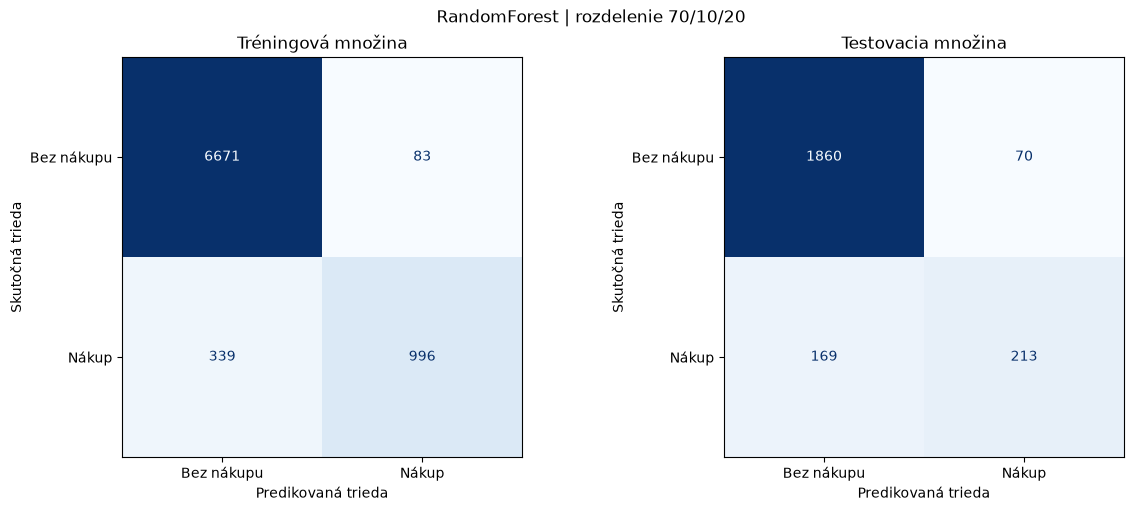
\includegraphics[width=\linewidth,height=0.78\textheight,keepaspectratio]{graf_24.png}
\end{center}

\begin{longtable}{>{\raggedright\arraybackslash}p{0.31000\linewidth}>{\raggedright\arraybackslash}p{0.18467\linewidth}>{\raggedright\arraybackslash}p{0.18467\linewidth}>{\raggedright\arraybackslash}p{0.18467\linewidth}}
 & precision & recall & f1-score \\
\hline
\endhead
Bez nákupu & 0.92 & 0.96 & 0.94 \\
Nákup & 0.75 & 0.56 & 0.64 \\
accuracy &  &  & 0.90 \\
macro avg & 0.83 & 0.76 & 0.79 \\
weighted avg & 0.89 & 0.90 & 0.89 \\
\end{longtable}

\begin{longtable}{>{\raggedright\arraybackslash}p{0.31000\linewidth}>{\raggedright\arraybackslash}p{0.62200\linewidth}}
 & support \\
\hline
\endhead
Bez nákupu & 1930 \\
Nákup & 382 \\
accuracy & 2312 \\
macro avg & 2312 \\
weighted avg & 2312 \\
\end{longtable}

Najlepším modelom podľa validácie bol Random Forest pri rozdelení 70/10/20, s validačnou accuracy 91.18\% a testovacou accuracy 89.66\%. Najvyššiu testovaciu accuracy dosiahol Random Forest pri 60/10/30 a to 89.71\% čo je rozdiel 0.05\%.

Najhorším modelom podľa validácie bola Logistic Regression pri 60/10/30, s validačnou accuracy 87.2\% a testovacou 87.6\%. Zachytila iba 36.3\% správne klasifikovaných nákupov.

Najlepšia konfigurácia Random Forestu mal maximálna hĺbka 10, počet zvažovaných vlastností 13 a minimálny počet vzoriek v liste 1. Jedna z najhorších mala maximálna hĺbka 5, počet zvažovaných vlastností 4 a minimálny počet vzoriek v liste 1, s validačnou accuracy 83.48\%. Takéto parametre vytvárajú plytké stromy, čo má za príčinu nedostatočné zachytávanie vzťahov v dátach.

Najväčší rozdiel medzi tréningom a testom mal Random Forest pri 80/10/10, kde trénovacia accuracy bola 96.62\% a testovacia 88.67\%, teda rozdiel 6.95. Pri 60/10/30 bol rozdiel iba 3.88. Výsledky z rozdelenia 80/10/10 naznačujú pretrénovanie.

Vybraný Random Forest správne rozpoznal 213 nákupov, ale 169 nákupov prehliadol pri testovaní. Precision bola 75.27\% (213/283) a recall 55.76\% (213/382) a F1 61.04\%.

Pri rovnakom rozdelení 70/10/20 prekonal Random Forest logistickú regresiu v accuracy o 2.03 ale recall až o 20.42.

\section*{Neural Network}

Rozdelenie: 70/15/15

Počet vstupov po predspracovaní: 72

Počty vzoriek: train 8089, val 1734, test 1734.

Podiel nákupov v tréningu: 16.52\%

\subsection*{net, Early\allowbreak{}Stopping a vyhodnotenie}

Používam plne prepojenú sieť s Re\allowbreak{}LU v skrytých vrstvách. Výstupný neurón vracia logit. BCEWith\allowbreak{}Logits\allowbreak{}Loss spája sigmoid a binárnu krížovú entropiu stabilne. Pri predikcii používam sigmoid a pevný prah 0.5. Adam aktualizuje váhy po minibatchoch. Všetky behy používajú rovnaký seed, batch size s 128 a maximálne 300 epoch. Dropout ani penalizáciu nepoužívam.

Early\allowbreak{}Stopping sleduje validačnú stratu. Ak počas 20 epoch nepríde zlepšenie väčšie než 0.0001 oproti poslednému významnému minimu, zastaví tréning. Obnoví váhy z absolútne najnižšej validačnej straty. Pri modeli bez Early\allowbreak{}Stoppingu hodnotím posledné váhy, aby sa pretrénovanie neskrylo obnovením skoršej epochy.

\subsection*{Kombinácie trénovania}

O demonštruje pretrénovanie veľkej siete s vrstvami 256, 128 a 64 neurónov pri learning rate 0.001 počas 300 epoch. ES opakuje rovnakú konfiguráciu ale pridáva Early\allowbreak{}Stopping.

E1-E3 menia learning rate pri rovnakých vrstvách 64 a 32 neurónov. E4 a E5 menia architektúru pri learning rate 0.001. Tým porovnávam 5 konfigurácií a aspoň 2 druhy nastavení.

Veľká sieť bez Early\allowbreak{}Stopping | epocha 1: tréningová strata 0.2882, validačná strata 0.3001

Veľká sieť bez Early\allowbreak{}Stopping | epocha 50: tréningová strata 0.0155, validačná strata 0.9478

Veľká sieť bez Early\allowbreak{}Stopping | epocha 100: tréningová strata 0.0029, validačná strata 1.3070

Veľká sieť bez Early\allowbreak{}Stopping | epocha 150: tréningová strata 0.0021, validačná strata 1.3768

Veľká sieť bez Early\allowbreak{}Stopping | epocha 200: tréningová strata 0.0007, validačná strata 1.3407

Veľká sieť bez Early\allowbreak{}Stopping | epocha 250: tréningová strata 0.0044, validačná strata 1.4861

Veľká sieť bez Early\allowbreak{}Stopping | epocha 300: tréningová strata 0.0012, validačná strata 1.1467

Veľká sieť bez Early\allowbreak{}Stopping: vykonaných 300 epoch, hodnotené váhy z epochy 300.

Veľká sieť s Early\allowbreak{}Stopping | epocha 1: tréningová strata 0.2882, validačná strata 0.3001

Veľká sieť s Early\allowbreak{}Stopping: vykonaných 26 epoch, hodnotené váhy z epochy 6.

E1 | epocha 1: tréningová strata 0.6273, validačná strata 0.6269

E1 | epocha 50: tréningová strata 0.2480, validačná strata 0.2701

E1 | epocha 100: tréningová strata 0.2232, validačná strata 0.2566

E1: vykonaných 149 epoch, hodnotené váhy z epochy 129.

E2 | epocha 1: tréningová strata 0.3488, validačná strata 0.3528

E2: vykonaných 34 epoch, hodnotené váhy z epochy 14.

E3 | epocha 1: tréningová strata 0.2563, validačná strata 0.2817

E3: vykonaných 25 epoch, hodnotené váhy z epochy 5.

E4 | epocha 1: tréningová strata 0.4568, validačná strata 0.4555

E4 | epocha 50: tréningová strata 0.2067, validačná strata 0.2542

E4: vykonaných 66 epoch, hodnotené váhy z epochy 46.

E5 | epocha 1: tréningová strata 0.3181, validačná strata 0.3255

E5: vykonaných 28 epoch, hodnotené váhy z epochy 8.

Hotovo: 7 tréningov na rozdelení 70/15/15

\subsection*{vyhodnotenie výsledkov a experimentov}

\begin{longtable}{>{\raggedright\arraybackslash}p{0.31000\linewidth}>{\raggedright\arraybackslash}p{0.18467\linewidth}>{\raggedright\arraybackslash}p{0.18467\linewidth}>{\raggedright\arraybackslash}p{0.18467\linewidth}}
Tréning & O & ES & E1 \\
\hline
\endhead
Skryté vrstvy & 256 \textrightarrow{} 128 \textrightarrow{} 64 & 256 \textrightarrow{} 128 \textrightarrow{} 64 & 64 \textrightarrow{} 32 \\
Learning rate & 0.0010 & 0.0010 & 0.0001 \\
Early\allowbreak{}Stopping & False & True & True \\
Vykonané epochy & 300 & 26 & 149 \\
Hodnotená epocha & 300 & 6 & 129 \\
Train accuracy (\%) & 99.9753 & 90.5180 & 90.9630 \\
Val accuracy (\%) & 87.6586 & 88.9273 & 89.5040 \\
Val loss & 1.1467 & 0.2578 & 0.2542 \\
Test accuracy (\%) & 86.8512 & 88.8697 & 89.0427 \\
Train balanced accuracy (\%) & 99.9251 & 83.1832 & 81.3783 \\
Test balanced accuracy (\%) & 73.8887 & 79.3062 & 77.3053 \\
Train F1 nákup & 0.9993 & 0.7156 & 0.7103 \\
Test F1 nákup & 0.5778 & 0.6584 & 0.6429 \\
Baseline train accuracy (\%) & 83.4837 & 83.4837 & 83.4837 \\
Baseline test accuracy (\%) & 83.5063 & 83.5063 & 83.5063 \\
Train-test rozdiel (p. b.) & 13.1241 & 1.6483 & 1.9204 \\
\end{longtable}

\begin{longtable}{>{\raggedright\arraybackslash}p{0.31000\linewidth}>{\raggedright\arraybackslash}p{0.18467\linewidth}>{\raggedright\arraybackslash}p{0.18467\linewidth}>{\raggedright\arraybackslash}p{0.18467\linewidth}}
Tréning & E2 & E3 & E4 \\
\hline
\endhead
Skryté vrstvy & 64 \textrightarrow{} 32 & 64 \textrightarrow{} 32 & 32 \\
Learning rate & 0.0010 & 0.0100 & 0.0010 \\
Early\allowbreak{}Stopping & True & True & True \\
Vykonané epochy & 34 & 25 & 66 \\
Hodnotená epocha & 14 & 5 & 46 \\
Train accuracy (\%) & 90.7281 & 90.9507 & 91.1979 \\
Val accuracy (\%) & 89.5617 & 89.3310 & 89.2157 \\
Val loss & 0.2541 & 0.2542 & 0.2533 \\
Test accuracy (\%) & 89.0427 & 88.9273 & 88.4660 \\
Train balanced accuracy (\%) & 82.1083 & 79.8999 & 81.2488 \\
Test balanced accuracy (\%) & 77.4456 & 75.1318 & 75.6974 \\
Train F1 nákup & 0.7115 & 0.6983 & 0.7136 \\
Test F1 nákup & 0.6442 & 0.6190 & 0.6183 \\
Baseline train accuracy (\%) & 83.4837 & 83.4837 & 83.4837 \\
Baseline test accuracy (\%) & 83.5063 & 83.5063 & 83.5063 \\
Train-test rozdiel (p. b.) & 1.6855 & 2.0233 & 2.7319 \\
\end{longtable}

\begin{longtable}{>{\raggedright\arraybackslash}p{0.31000\linewidth}>{\raggedright\arraybackslash}p{0.62200\linewidth}}
Tréning & E5 \\
\hline
\endhead
Skryté vrstvy & 128 \textrightarrow{} 64 \textrightarrow{} 32 \\
Learning rate & 0.0010 \\
Early\allowbreak{}Stopping & True \\
Vykonané epochy & 28 \\
Hodnotená epocha & 8 \\
Train accuracy (\%) & 90.4067 \\
Val accuracy (\%) & 88.6967 \\
Val loss & 0.2559 \\
Test accuracy (\%) & 88.6967 \\
Train balanced accuracy (\%) & 84.4375 \\
Test balanced accuracy (\%) & 80.3249 \\
Train F1 nákup & 0.7223 \\
Test F1 nákup & 0.6644 \\
Baseline train accuracy (\%) & 83.4837 \\
Baseline test accuracy (\%) & 83.5063 \\
Train-test rozdiel (p. b.) & 1.7101 \\
\end{longtable}

Najlepší experiment podľa validácie: E2

Najhorší experiment podľa validácie: E5

Bez Early\allowbreak{}Stopping: minimum val loss 0.2578 v epoche 6, na konci 1.1467.

Train loss v rovnakých epochách: 0.2085 \textrightarrow{} 0.0012.

Early\allowbreak{}Stopping obnovil epochu 6 po 26 vykonaných epochách.

Rozdiel train-test pred/po Early\allowbreak{}Stopping (p. b.): 13.12 1.65

\begin{longtable}{>{\raggedright\arraybackslash}p{0.31000\linewidth}>{\raggedright\arraybackslash}p{0.18467\linewidth}>{\raggedright\arraybackslash}p{0.18467\linewidth}>{\raggedright\arraybackslash}p{0.18467\linewidth}}
Množina & Loss & Accuracy (\%) & Balanced accuracy (\%) \\
\hline
\endhead
train & 0.0012 & 99.9753 & 99.9251 \\
test & 1.3414 & 86.8512 & 73.8887 \\
\end{longtable}

\begin{longtable}{>{\raggedright\arraybackslash}p{0.31000\linewidth}>{\raggedright\arraybackslash}p{0.29400\linewidth}>{\raggedright\arraybackslash}p{0.29400\linewidth}}
Množina & F1 nákup & Baseline accuracy (\%) \\
\hline
\endhead
train & 0.9993 & 83.4837 \\
test & 0.5778 & 83.5063 \\
\end{longtable}

\begin{center}
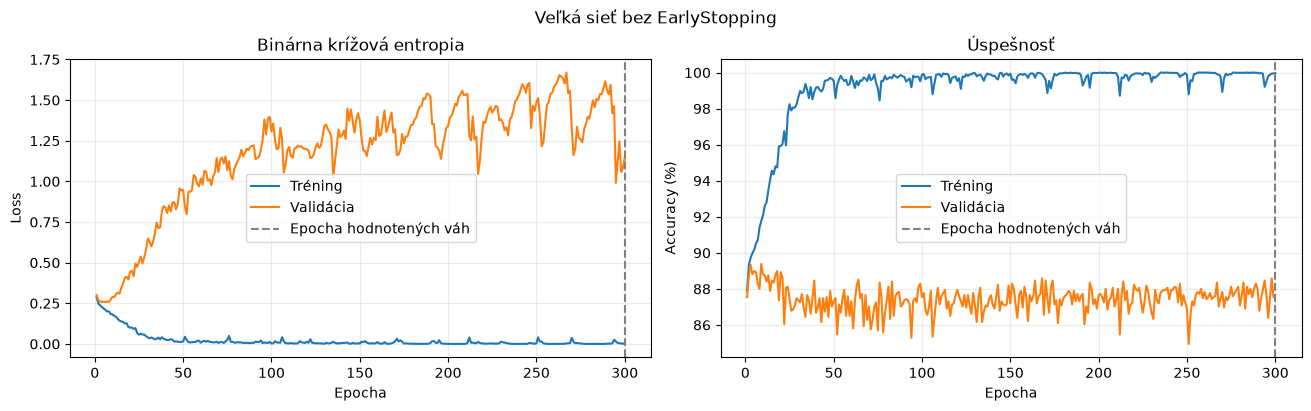
\includegraphics[width=\linewidth,height=0.78\textheight,keepaspectratio]{graf_25.png}
\end{center}

\begin{center}
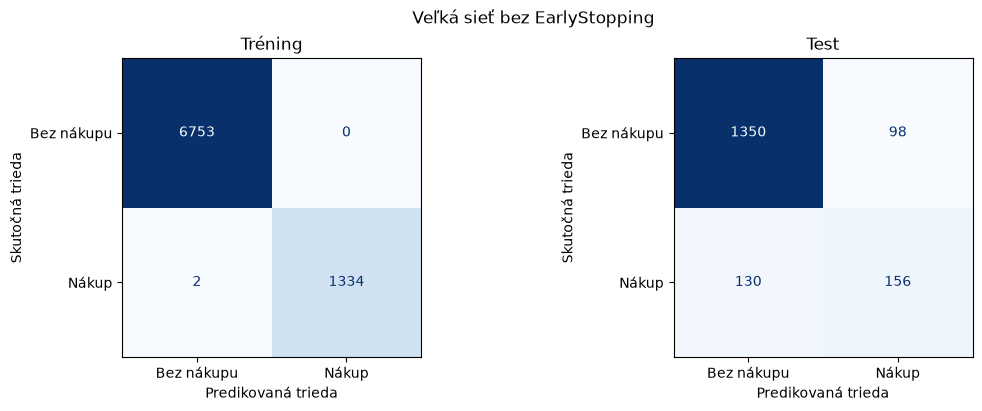
\includegraphics[width=\linewidth,height=0.78\textheight,keepaspectratio]{graf_26.png}
\end{center}

Veľká sieť bez Early\allowbreak{}Stopping – train

\begin{longtable}{>{\raggedright\arraybackslash}p{0.31000\linewidth}>{\raggedright\arraybackslash}p{0.18467\linewidth}>{\raggedright\arraybackslash}p{0.18467\linewidth}>{\raggedright\arraybackslash}p{0.18467\linewidth}}
 & precision & recall & f1-score \\
\hline
\endhead
Bez nákupu & 1.00 & 1.00 & 1.00 \\
Nákup & 1.00 & 1.00 & 1.00 \\
accuracy &  &  & 1.00 \\
macro avg & 1.00 & 1.00 & 1.00 \\
weighted avg & 1.00 & 1.00 & 1.00 \\
\end{longtable}

\begin{longtable}{>{\raggedright\arraybackslash}p{0.31000\linewidth}>{\raggedright\arraybackslash}p{0.62200\linewidth}}
 & support \\
\hline
\endhead
Bez nákupu & 6753 \\
Nákup & 1336 \\
accuracy & 8089 \\
macro avg & 8089 \\
weighted avg & 8089 \\
\end{longtable}

Veľká sieť bez Early\allowbreak{}Stopping – test

\begin{longtable}{>{\raggedright\arraybackslash}p{0.31000\linewidth}>{\raggedright\arraybackslash}p{0.18467\linewidth}>{\raggedright\arraybackslash}p{0.18467\linewidth}>{\raggedright\arraybackslash}p{0.18467\linewidth}}
 & precision & recall & f1-score \\
\hline
\endhead
Bez nákupu & 0.91 & 0.93 & 0.92 \\
Nákup & 0.61 & 0.55 & 0.58 \\
accuracy &  &  & 0.87 \\
macro avg & 0.76 & 0.74 & 0.75 \\
weighted avg & 0.86 & 0.87 & 0.87 \\
\end{longtable}

\begin{longtable}{>{\raggedright\arraybackslash}p{0.31000\linewidth}>{\raggedright\arraybackslash}p{0.62200\linewidth}}
 & support \\
\hline
\endhead
Bez nákupu & 1448 \\
Nákup & 286 \\
accuracy & 1734 \\
macro avg & 1734 \\
weighted avg & 1734 \\
\end{longtable}

\begin{longtable}{>{\raggedright\arraybackslash}p{0.31000\linewidth}>{\raggedright\arraybackslash}p{0.18467\linewidth}>{\raggedright\arraybackslash}p{0.18467\linewidth}>{\raggedright\arraybackslash}p{0.18467\linewidth}}
Množina & Loss & Accuracy (\%) & Balanced accuracy (\%) \\
\hline
\endhead
train & 0.2085 & 90.5180 & 83.1832 \\
test & 0.2611 & 88.8697 & 79.3062 \\
\end{longtable}

\begin{longtable}{>{\raggedright\arraybackslash}p{0.31000\linewidth}>{\raggedright\arraybackslash}p{0.29400\linewidth}>{\raggedright\arraybackslash}p{0.29400\linewidth}}
Množina & F1 nákup & Baseline accuracy (\%) \\
\hline
\endhead
train & 0.7156 & 83.4837 \\
test & 0.6584 & 83.5063 \\
\end{longtable}

\begin{center}
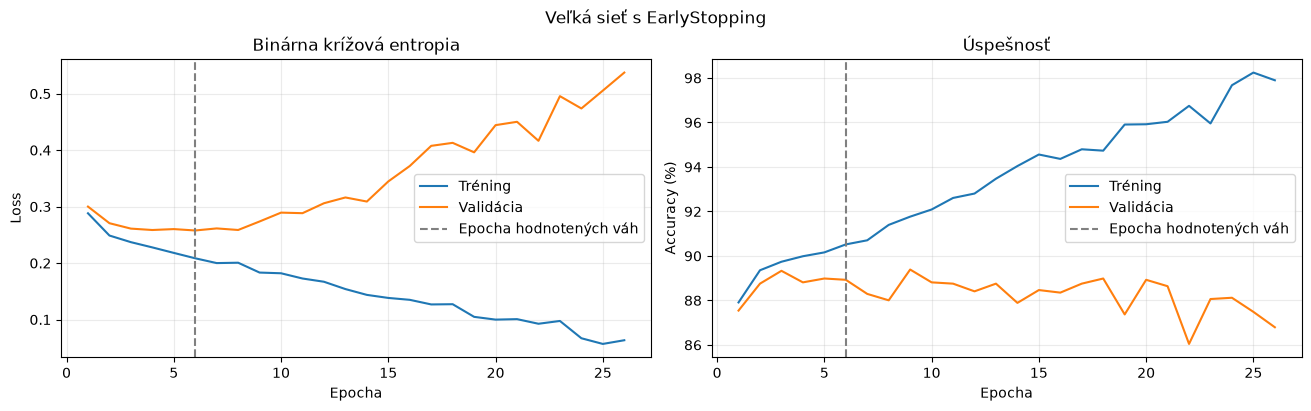
\includegraphics[width=\linewidth,height=0.78\textheight,keepaspectratio]{graf_27.png}
\end{center}

\begin{center}
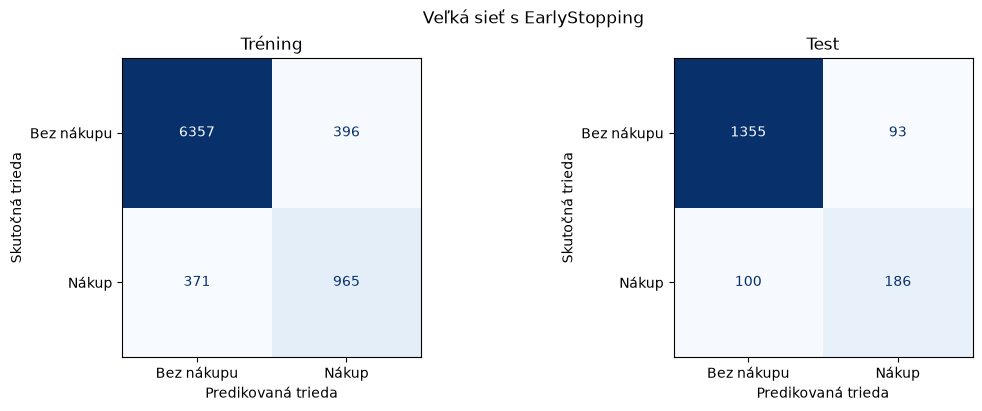
\includegraphics[width=\linewidth,height=0.78\textheight,keepaspectratio]{graf_28.png}
\end{center}

Veľká sieť s Early\allowbreak{}Stopping – train

\begin{longtable}{>{\raggedright\arraybackslash}p{0.31000\linewidth}>{\raggedright\arraybackslash}p{0.18467\linewidth}>{\raggedright\arraybackslash}p{0.18467\linewidth}>{\raggedright\arraybackslash}p{0.18467\linewidth}}
 & precision & recall & f1-score \\
\hline
\endhead
Bez nákupu & 0.94 & 0.94 & 0.94 \\
Nákup & 0.71 & 0.72 & 0.72 \\
accuracy &  &  & 0.91 \\
macro avg & 0.83 & 0.83 & 0.83 \\
weighted avg & 0.91 & 0.91 & 0.91 \\
\end{longtable}

\begin{longtable}{>{\raggedright\arraybackslash}p{0.31000\linewidth}>{\raggedright\arraybackslash}p{0.62200\linewidth}}
 & support \\
\hline
\endhead
Bez nákupu & 6753 \\
Nákup & 1336 \\
accuracy & 8089 \\
macro avg & 8089 \\
weighted avg & 8089 \\
\end{longtable}

Veľká sieť s Early\allowbreak{}Stopping – test

\begin{longtable}{>{\raggedright\arraybackslash}p{0.31000\linewidth}>{\raggedright\arraybackslash}p{0.18467\linewidth}>{\raggedright\arraybackslash}p{0.18467\linewidth}>{\raggedright\arraybackslash}p{0.18467\linewidth}}
 & precision & recall & f1-score \\
\hline
\endhead
Bez nákupu & 0.93 & 0.94 & 0.93 \\
Nákup & 0.67 & 0.65 & 0.66 \\
accuracy &  &  & 0.89 \\
macro avg & 0.80 & 0.79 & 0.80 \\
weighted avg & 0.89 & 0.89 & 0.89 \\
\end{longtable}

\begin{longtable}{>{\raggedright\arraybackslash}p{0.31000\linewidth}>{\raggedright\arraybackslash}p{0.62200\linewidth}}
 & support \\
\hline
\endhead
Bez nákupu & 1448 \\
Nákup & 286 \\
accuracy & 1734 \\
macro avg & 1734 \\
weighted avg & 1734 \\
\end{longtable}

\begin{longtable}{>{\raggedright\arraybackslash}p{0.31000\linewidth}>{\raggedright\arraybackslash}p{0.18467\linewidth}>{\raggedright\arraybackslash}p{0.18467\linewidth}>{\raggedright\arraybackslash}p{0.18467\linewidth}}
Množina & Loss & Accuracy (\%) & Balanced accuracy (\%) \\
\hline
\endhead
train & 0.2159 & 90.7281 & 82.1083 \\
test & 0.2596 & 89.0427 & 77.4456 \\
\end{longtable}

\begin{longtable}{>{\raggedright\arraybackslash}p{0.31000\linewidth}>{\raggedright\arraybackslash}p{0.29400\linewidth}>{\raggedright\arraybackslash}p{0.29400\linewidth}}
Množina & F1 nákup & Baseline accuracy (\%) \\
\hline
\endhead
train & 0.7115 & 83.4837 \\
test & 0.6442 & 83.5063 \\
\end{longtable}

\begin{center}
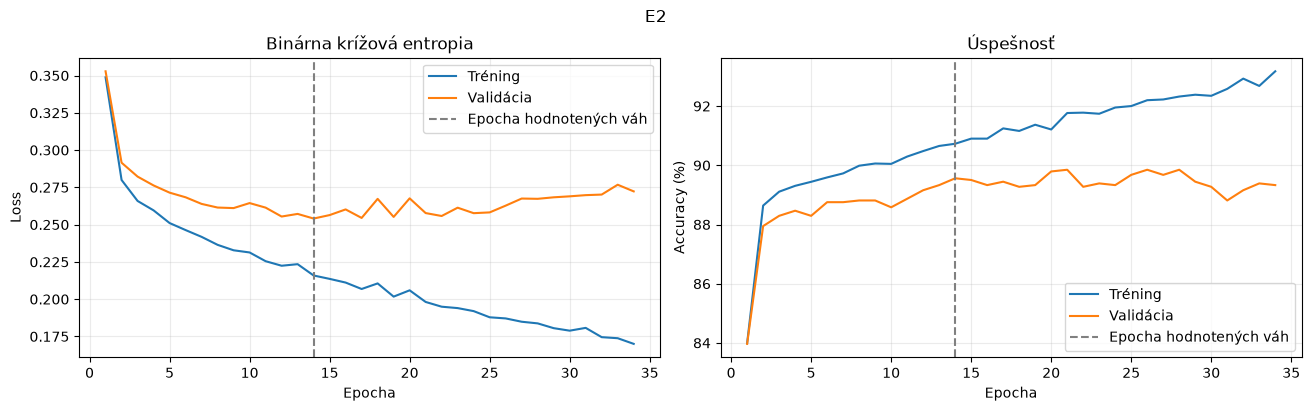
\includegraphics[width=\linewidth,height=0.78\textheight,keepaspectratio]{graf_29.png}
\end{center}

\begin{center}
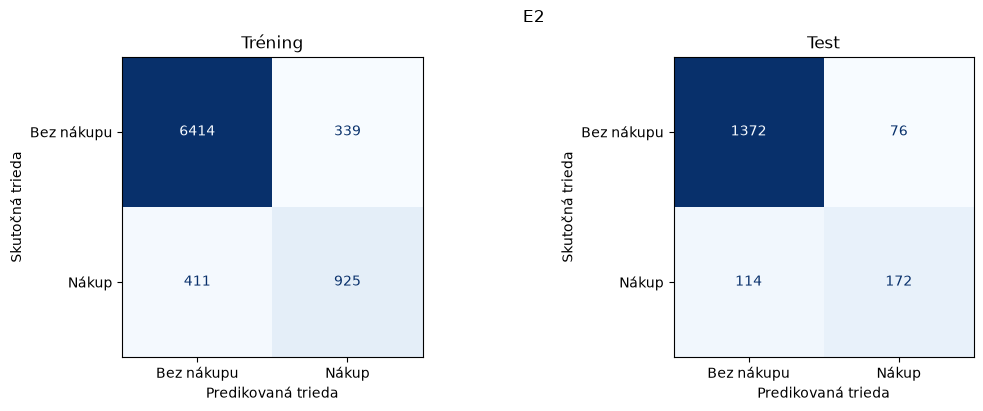
\includegraphics[width=\linewidth,height=0.78\textheight,keepaspectratio]{graf_30.png}
\end{center}

E2 – train

\begin{longtable}{>{\raggedright\arraybackslash}p{0.31000\linewidth}>{\raggedright\arraybackslash}p{0.18467\linewidth}>{\raggedright\arraybackslash}p{0.18467\linewidth}>{\raggedright\arraybackslash}p{0.18467\linewidth}}
 & precision & recall & f1-score \\
\hline
\endhead
Bez nákupu & 0.94 & 0.95 & 0.94 \\
Nákup & 0.73 & 0.69 & 0.71 \\
accuracy &  &  & 0.91 \\
macro avg & 0.84 & 0.82 & 0.83 \\
weighted avg & 0.91 & 0.91 & 0.91 \\
\end{longtable}

\begin{longtable}{>{\raggedright\arraybackslash}p{0.31000\linewidth}>{\raggedright\arraybackslash}p{0.62200\linewidth}}
 & support \\
\hline
\endhead
Bez nákupu & 6753 \\
Nákup & 1336 \\
accuracy & 8089 \\
macro avg & 8089 \\
weighted avg & 8089 \\
\end{longtable}

E2 – test

\begin{longtable}{>{\raggedright\arraybackslash}p{0.31000\linewidth}>{\raggedright\arraybackslash}p{0.18467\linewidth}>{\raggedright\arraybackslash}p{0.18467\linewidth}>{\raggedright\arraybackslash}p{0.18467\linewidth}}
 & precision & recall & f1-score \\
\hline
\endhead
Bez nákupu & 0.92 & 0.95 & 0.94 \\
Nákup & 0.69 & 0.60 & 0.64 \\
accuracy &  &  & 0.89 \\
macro avg & 0.81 & 0.77 & 0.79 \\
weighted avg & 0.89 & 0.89 & 0.89 \\
\end{longtable}

\begin{longtable}{>{\raggedright\arraybackslash}p{0.31000\linewidth}>{\raggedright\arraybackslash}p{0.62200\linewidth}}
 & support \\
\hline
\endhead
Bez nákupu & 1448 \\
Nákup & 286 \\
accuracy & 1734 \\
macro avg & 1734 \\
weighted avg & 1734 \\
\end{longtable}

\begin{longtable}{>{\raggedright\arraybackslash}p{0.31000\linewidth}>{\raggedright\arraybackslash}p{0.18467\linewidth}>{\raggedright\arraybackslash}p{0.18467\linewidth}>{\raggedright\arraybackslash}p{0.18467\linewidth}}
Množina & Loss & Accuracy (\%) & Balanced accuracy (\%) \\
\hline
\endhead
train & 0.2176 & 90.4067 & 84.4375 \\
test & 0.2607 & 88.6967 & 80.3249 \\
\end{longtable}

\begin{longtable}{>{\raggedright\arraybackslash}p{0.31000\linewidth}>{\raggedright\arraybackslash}p{0.29400\linewidth}>{\raggedright\arraybackslash}p{0.29400\linewidth}}
Množina & F1 nákup & Baseline accuracy (\%) \\
\hline
\endhead
train & 0.7223 & 83.4837 \\
test & 0.6644 & 83.5063 \\
\end{longtable}

\begin{center}
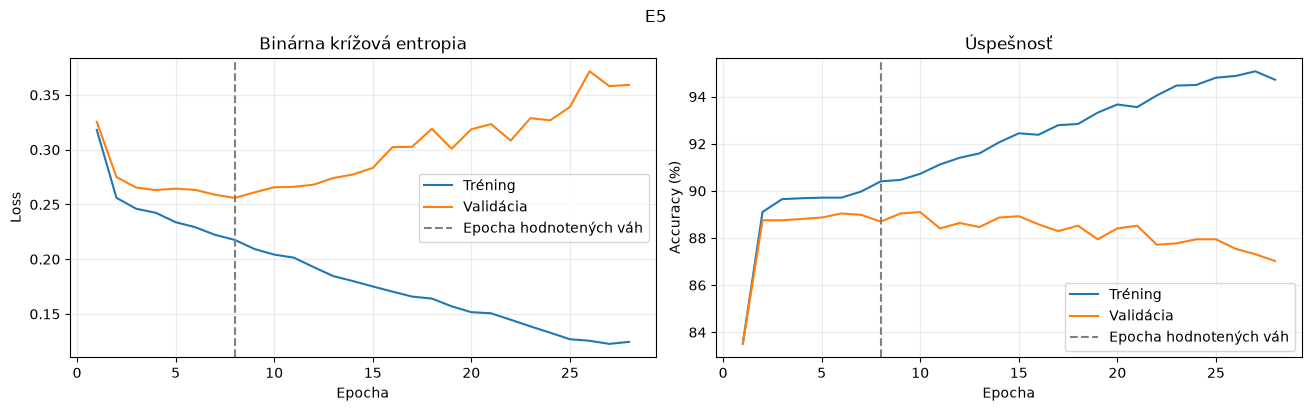
\includegraphics[width=\linewidth,height=0.78\textheight,keepaspectratio]{graf_31.png}
\end{center}

\begin{center}
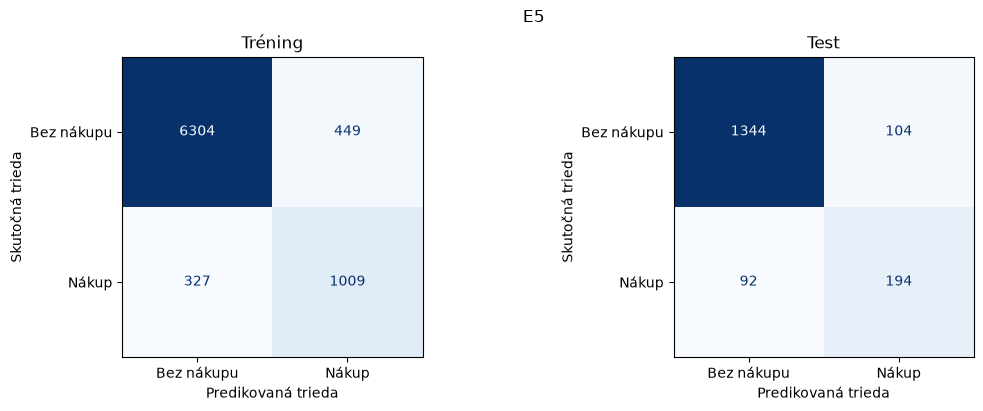
\includegraphics[width=\linewidth,height=0.78\textheight,keepaspectratio]{graf_32.png}
\end{center}

E5 – train

\begin{longtable}{>{\raggedright\arraybackslash}p{0.31000\linewidth}>{\raggedright\arraybackslash}p{0.18467\linewidth}>{\raggedright\arraybackslash}p{0.18467\linewidth}>{\raggedright\arraybackslash}p{0.18467\linewidth}}
 & precision & recall & f1-score \\
\hline
\endhead
Bez nákupu & 0.95 & 0.93 & 0.94 \\
Nákup & 0.69 & 0.76 & 0.72 \\
accuracy &  &  & 0.90 \\
macro avg & 0.82 & 0.84 & 0.83 \\
weighted avg & 0.91 & 0.90 & 0.91 \\
\end{longtable}

\begin{longtable}{>{\raggedright\arraybackslash}p{0.31000\linewidth}>{\raggedright\arraybackslash}p{0.62200\linewidth}}
 & support \\
\hline
\endhead
Bez nákupu & 6753 \\
Nákup & 1336 \\
accuracy & 8089 \\
macro avg & 8089 \\
weighted avg & 8089 \\
\end{longtable}

E5 – test

\begin{longtable}{>{\raggedright\arraybackslash}p{0.31000\linewidth}>{\raggedright\arraybackslash}p{0.18467\linewidth}>{\raggedright\arraybackslash}p{0.18467\linewidth}>{\raggedright\arraybackslash}p{0.18467\linewidth}}
 & precision & recall & f1-score \\
\hline
\endhead
Bez nákupu & 0.94 & 0.93 & 0.93 \\
Nákup & 0.65 & 0.68 & 0.66 \\
accuracy &  &  & 0.89 \\
macro avg & 0.79 & 0.80 & 0.80 \\
weighted avg & 0.89 & 0.89 & 0.89 \\
\end{longtable}

\begin{longtable}{>{\raggedright\arraybackslash}p{0.31000\linewidth}>{\raggedright\arraybackslash}p{0.62200\linewidth}}
 & support \\
\hline
\endhead
Bez nákupu & 1448 \\
Nákup & 286 \\
accuracy & 1734 \\
macro avg & 1734 \\
weighted avg & 1734 \\
\end{longtable}

Neurónovú sieť som trénoval na rozdelení 70 \% tréningových, 15 \% validačných a 15 \% testovacích dát. Všetkých sedem tréningov používalo rovnaké vzorky a predspracovanie naučené iba na tréningovej množine. Výsledky sú preto medzi jednotlivými konfiguráciami porovnateľné. Validáciu som použil na Early\allowbreak{}Stopping a výber konfigurácie, testovacie dáta na záverečné vyhodnotenie.

Pri veľkej sieti bez Early\allowbreak{}Stopping sa jasne prejavilo pretrénovanie. Tréningová strata postupne klesala takmer k nule a tréningová accuracy dosiahla 99,98 \%. Validačná strata však po minime v 6. epoche začala rásť. Sieť sa teda stále lepšie prispôsobovala tréningovým príkladom, ale jej schopnosť pracovať s nevidenými dátami sa zhoršovala. Potvrdila to testovacia accuracy 86,85 \%, ktorá bola oproti tréningovej nižšia o 13,12 percentuálneho bodu. Tréningová konfúzna matica mala takmer všetky predikcie na diagonále, zatiaľ čo testovacia obsahovala podstatne viac nesprávnych predikcií.

Early\allowbreak{}Stopping výrazne obmedzil pretrénovanie. Pri rovnakej architektúre zastavil tréning po 26 epochách a obnovil váhy zo 6. epochy, v ktorej bola validačná strata najnižšia. Tréningová accuracy klesla na 90,52 \%, ale testovacia sa zvýšila na 88,87 \%. Rozdiel medzi nimi sa zmenšil na 1,65 percentuálneho bodu. Zlepšila sa aj testovacia balanced accuracy a F1 nákupov. Nižšia tréningová úspešnosť teda predstavovala prijateľný kompromis za lepšiu generalizáciu. Graf stále zobrazuje zhoršovanie počas ďalších epoch čakania, no výsledné metriky a konfúzne matice patria obnoveným váham zo 6. epochy.

V experimentoch E1–E5 som menil rýchlosť učenia a architektúru siete. Podľa validačnej accuracy bol najlepší E2, ktorý používal skryté vrstvy so 64 a 32 neurónmi a learning rate 0,001. Dosiahol tréningovú accuracy 90,73 \%, validačnú 89,56 \% a testovaciu 89,04 \%. E1 dosiahol rovnakú testovaciu accuracy, ale potreboval 149 epoch oproti 34 pri E2. Vyšší learning rate v E3 skrátil tréning, no nepriniesol lepšiu testovaciu úspešnosť. Ani zmena veľkosti siete nezaručila zlepšenie, preto väčšia kapacita sama osebe nie je dôvodom na výber modelu.

Konfúzna matica E2 ukazuje, že sieť správne rozpoznáva obe triedy, ale úspešnejšia je pri návštevách bez nákupu. Na teste správne označila 1 372 návštev bez nákupu a 172 nákupov. Zároveň nesprávne predikovala nákup pri 76 návštevách a nezachytila 114 skutočných nákupov. Zachytila teda približne 60,14 \% nákupov. Výrazná diagonála potvrdzuje užitočnosť modelu, ale accuracy blízka 90 \% neznamená, že sieť rozpoznáva takmer všetky nákupy.

Podľa validačnej accuracy bol najhorší E5, jeho výsledky však ukazujú význam sledovania viacerých metrík. Mal nižšiu testovaciu accuracy než E2, ale vyššiu balanced accuracy aj F1 nákupov. Označenie „najhorší“ preto platí iba pre zvolené validačné kritérium. Ak by hlavným cieľom bolo zachytiť viac nákupov, bolo by vhodné vopred zvoliť tomu zodpovedajúcu validačnú metriku.

Za výslednú konfiguráciu pri použitom kritériu považujem E2. Prekonala väčšinový baseline s testovacou accuracy 83,51 \% a vykazovala podstatne menší rozdiel medzi tréningom a testom než zámerne pretrénovaná sieť. Výsledky podporujú použitie Early\allowbreak{}Stopping a ukazujú, že vhodná kombinácia architektúry a rýchlosti učenia je dôležitejšia než samotné zväčšovanie siete. Rozdiely medzi experimentmi sú však malé a pochádzajú z jediného rozdelenia a seedu, preto ich nemožno považovať za dôkaz všeobecnej nadradenosti jednej konfigurácie.

\end{document}
